\documentclass[12pt, letterpaper, oneside]{book}
%\documentclass[12pt, letterpaper]{book}

\usepackage[spanish,es-tabla]{babel}
\usepackage[utf8x]{inputenc}
\usepackage{mathtools}
\usepackage{microtype}
\usepackage{emptypage}
\usepackage{usmtesis}
\usepackage{url}
\usepackage{caption}
\usepackage{amsmath}
\usepackage{listings}
\usepackage{graphicx}
\usepackage{subfigure}
%\usepackage{subcaption}
\usepackage{cite}
\usepackage{rotating}
\usepackage{amsfonts}
\usepackage{hyperref}
\usepackage{algorithm}
\usepackage{algorithmic}
\usepackage{float}
\usepackage{comment}
\usepackage{lscape}

\usepackage{tikz}
\usetikzlibrary{babel,arrows.meta,shapes,arrows}

\usepackage{afterpage}

\newcommand\blankpage{%
    \null
    \thispagestyle{empty}%
    %\addtocounter{page}{-1}%
    \newpage}

%\usepackage{layout} %debug only

\RequirePackage{fancyhdr}
\newcommand{\hsp}[1][20]{\hspace{#1pt}}
\fancyhf{}
\fancypagestyle{plain}{%
	\fancyhf{} 
	\fancyhead[L]{\scriptsize \rightmark}
	\fancyhead[R]{\scriptsize \leftmark}
	\fancyfoot[R]{\bfseries \thepage}
	\fancyfoot[L]{Departamento de Informática. UTFSM.}
	\renewcommand{\headrulewidth}{0.1pt}
	\renewcommand{\footrulewidth}{0.1pt}
}
%\setlength{\footheight}{110pt} 

%macros
\renewcommand{\tt}[1]{\texttt{#1}}
\renewcommand{\bf}[1]{\textbf{#1}}
\newcommand{\etal}{\emph{et al.}}

\begin{document}
\frontmatter
\thispagestyle{empty}
%!TEX root = main.tex

\begin{center}
  \begin{spacing}{1}
    {\large UNIVERSIDAD TÉCNICA FEDERICO SANTA MARÍA}\\
    DEPARTAMENTO DE INFORMÁTICA\\
    VALPARAÍSO - CHILE
  \end{spacing}

  \vspace{12mm}
  
\includegraphics[height=50mm]{figures/usm_logo.png}
  \vspace{15mm}

  \begin{spacing}{1.5} 
    \textbf{\large \emph{Particle Swarm Optimization} para el ajuste de modelos
      probabilísticos a datos del viento en Valparaíso}\\
    %\textbf{\large asd}\\
  \end{spacing}

  \vspace{20mm}
  \textbf{\large ALONSO JAVIER SANDOVAL ACEVEDO}
  \vspace{12mm}

  \begin{spacing}{1.25} 
    MEMORIA PARA OPTAR AL TÍTULO DE\\
    INGENIERO CIVIL EN INFORMÁTICA
    %PRIMER AVANCE DE MEMORIA
  \end{spacing}

  \vspace{15mm}
  \begin{table}[h]
    \begin{center}
      \begin{tabular}{ l c l }
        PROFESOR GUÍA & : & MARÍA CRISTINA RIFF.\\
        PROFESOR CORREFERENTE & : & X. X.\\
      \end{tabular}
    \end{center}
  \end{table}

  \vfill
  \large JULIO 2016
\end{center}

\newpage
\chapter*{ }
\vspace{-3cm}
\newpage

%debug
%\layout
%\newpage

%% Hack para el abstract corregir si se puede.
\chapter*{ }
\vspace{-3cm}
\section*{Resumen}\chaptermark{Abstract}
La velocidad y la dirección del viento son factores esenciales en el estudio de este fenómeno meteorológico. Diversos trabajos realizados en las áreas de energía eólica, medio ambiente y desastres naturales proponen métodos para modelar estas características del viento. La distribución de Weibull es ampliamente utilizada para modelar la velocidad, mientras que la mezcla de distribuciones de von Mises es sugerida para la dirección. Comúnmente, para el ajuste de los parámetros de estas distribuciones a ciertos datos recolectados, se utilizan métodos numéricos, sin embargo, estos pueden presentar deficiencias en cuanto a tiempos de ejecución o calidad de solución. En esta memoria, se implementa la meta-heurística \emph{Particle Swarm Optimization} para el ajuste de los parámetros de las distribuciones mencionadas a los datos del viento de la comuna de Valparaíso. Esta técnica provee de buenas soluciones en cortos tiempos de ejecución, siendo adaptable para el ajuste de ambas distribuciones. Además, se propone una estrategia para el control de la convergencia prematura del PSO, mejorando el trabajo realizado a la fecha.
\section*{Abstact}
The speed and direction of the wind are essential factors in the study of this meteorological phenomenon. Many works performed in the areas of wind energy, environment and natural disasters propose methods to model these wind properties. The Weibull distribution is widely used to model velocity, while the mixture of von Mises distribution is suggested for direction. Commonly, numerical methods are used for the adjustment of the parameters of these distributions to certain data collected, however, these can present deficiencies in terms of execution times or solution quality. In this study, the meta-heuristic Particle Swarm Optimization is implemented for the adjustment of the parameters of the mentioned distributions to the data of wind of the commune of Valparaiso. This technique provides good solutions in short execution times, being adaptable for the adjustment of both distributions. Furthermore, a strategy is proposed for the control of the premature convergence of the PSO algorithm, improving the work done to date.
\newpage
\chapter*{ }\chaptermark{ }
\vspace{-3cm}
\newpage

\begin{spacing}{1}
\chaptermark{Tabla de contenidos}
\tableofcontents
\listoffigures
\listoftables
\end{spacing}

\mainmatter

%!TEX root = main.tex

\chapter{Introducción}

\section{Identificación del problema}
El viento es uno de los fenómenos metereológicos más comunes de las zonas costeras de Valparaíso. Sus características afectan distintos aspectos del entorno que influyen en nuestras vidas, como las condiciones del clima, la sensación térmica, algunos desastres naturales, entre otros. Esto atrae el interés de los especialistas, fomentando la investigación para lograr controlar, en cierta medida, las distintas variables que condicionan su comportamiento, de manera de poder predecir los fenómenos subyacentes a este. Más aún, el viento es ampliamente conocido por ser una fuente renovable y poco contaminante de energía, comunmente llamada energía eólica, lo que hace aún más interesante y necesario el estudio de este fenómeno metereológico.\\
En los últimos años, tanto el gobierno de Chile como la ciudadanía, han mostrado un creciente interés en las fuentes de energías renovables y con mínimo impacto ambiental, por lo que distintos proyectos en la matería han sido llevados a cabo, desde estudios de factibilidad y recopilación de datos hasta el emplazamiento de las primeras centrales de fuentes de energía límpia. El año 2014, el ministerio de energía publicó un extenso reporte acerca de la situación actual del país en materias de energías renovables, en donde se pueden ver distintas proyecciones y estimaciones de implementación de posibles plantas de generación a lo largo del país. \cite{minenergia14}\\
Cualquiera sea el estudio de las condiciones climáticas del viento para predecir su potencial energético, existen dos variables fundamentales ha considerar para obtener estas predicciones: la velocidad y la dirección del viento. Actualmente, estos datos están disponibles y son obtenidos por diversos centros metereológicos a lo largo del país, en partícular, el servicio metereológico de la Armada de Chile, que cuenta con el equipo necesario para registrar el comportamiento del viento al lo largo de las distintas épocas del año y en diferentes zonas de Chile.\\
Si bien la obtención de los datos es un paso, para poder obtener información o conocimiento relevante sobre estos (algo más que un promedio, por ejemplo), es necesario generar modelos que permitan ``explicar'' la distribución de datos y de cierta forma predecir el comportamiento futuro del viento. En la literatura, son ampliamente aceptadas la distribución de \emph{Weibull} para modelar el conjunto datos de velocidad y la distribución de Von Mises para el modelo de la dirección del viento. Ambas distribuciones probabilísticas requieren de la determinación de parámetros para que el modelo se ajuste a los datos obtenidos. Comunmente, se utilizan métodos númericos para la determinación de estos parámetros, sin embargo, estudios recientes han demostrado que la utilización de algorítmos basados en la metaheurística \emph{Particle Swarm Optimization} mejoran los parámetros obtenidos por los métodos tradicionales y por ende la aproximación del modelo al comportamiento real.\\ 

\section{Objetivos}
Aplicar métodos actuales de optimización basados en la metaheurística \emph{Particle Swarm Optimization} para el ajuste de modelos probabilísticos de dirección y velocidad del viento a los datos recopilados del viento en Valparaíso, con el fin de presentar resultados que permitan inferir información precisa acerca de las condiciones de la región para la generación de energía eólica y otras potenciales aplicaciones.

\subsection{Objetivos específicos}
\begin{enumerate}
    \item Implementar un algoritmo basado en \emph{Particle Optimization Sworm} para \textbf{encontrar} los parámetros de un modelo probabilístico que se ajusten a los datos de la velocidad del viento en Valparaíso. 
    \item Implementar un algoritmo basado en \emph{Particle Optimization Sworm} para \textbf{optimizar} los parámetros de un modelo probabilístico que se ajusten a los datos de la dirección del viento en Valparaíso.
    \item Evaluar los modelos sobre los datos del viento para validar la propuesta realizada.
\end{enumerate}


%!TEX root = main.tex

\chapter{Estado del arte}
\section{Particle Swarm Optimization}
Como se introduce en el artículo de Kaveh \cite{Psoexplain14}, el algoritmo \emph{Particle Swarm Optimization} es una meta-heurística inspirada en las observaciones de la naturaleza acerca del comportamiento social de poblaciones de enjambres. Esta abstracción está basada, por ejemplo, en las gaviotas, las cuales suelen moverse en grupos, conocidos como bandadas, cerca del mar en búsqueda de zonas donde hayan alimento (peces). El método simula la conducta de los individuos a través de partículas que se mueven dentro de un espacio (de búsqueda), siendo estas afectadas por factores individuales (conocimiento propio) y colectivos (conocimiento del enjambre), los cuales dirigen el movimiento de estos grupos a ciertas zonas las que son determinadas por una función objetivo (\emph{fitness function}).\\
Para cada partícula su vector posición  $\vec{x}$ representa una solución candidata, la cual varía dentro del espacio de búsqueda a velocidad $\vec{v}$. Después de varias iteraciones, el enjambre o conjunto de partículas, se irá concentrando en aquellas zonas donde la posición obtenga mejores valores para la función objetivo.
\\El modelo clásico presentado por Kennedy y Eberhart\cite{Kennedy95}, describe la variación de la velocidad y de la posición de las partículas como se presenta a continuación:
\begin{align}
    v_{i,j}^{k+1} &= v_{i,j}^{k} + c_{1}r_{1}(xbest_{i,j}^k - x_{i,j}^k) + c_{2}r_{2}(xgbest_{j}^{k} - x_{i,j}^k) \\
    x_{i,j}^{k+1} &= x_{i,j}^{k} + v_{i,j}^{k+1}
\end{align}    
Como se explica en Kaveh \cite{Psoexplain14} $x_{i,j}^{k}$ y $v_{i,j}^{k}$ son la $j$-ésima componente de la posición y la velocidad de la partícula $i$ respectivamente en la iteración o tiempo $k$, $r_{1}$ y $r_{2}$ son número aleatorios uniformes que varían de 0 a 1, $xbest_i$ y $xgbest$ representan las mejores soluciones alcanzadas por la partícula y por el enjambre respectivamente, $c_1$ y $c_2$ son parámetros que representan la confianza en la solución individual de la partícula (parámetro cognitivo) y la incidencia del aspecto colectivo o solución global (parámetro social), respectivamente. Un esquema de la interacción de estos componentes se aprecia en la figura \ref{fig:move_part}\\
\begin{figure}[h!]
    \centering    
    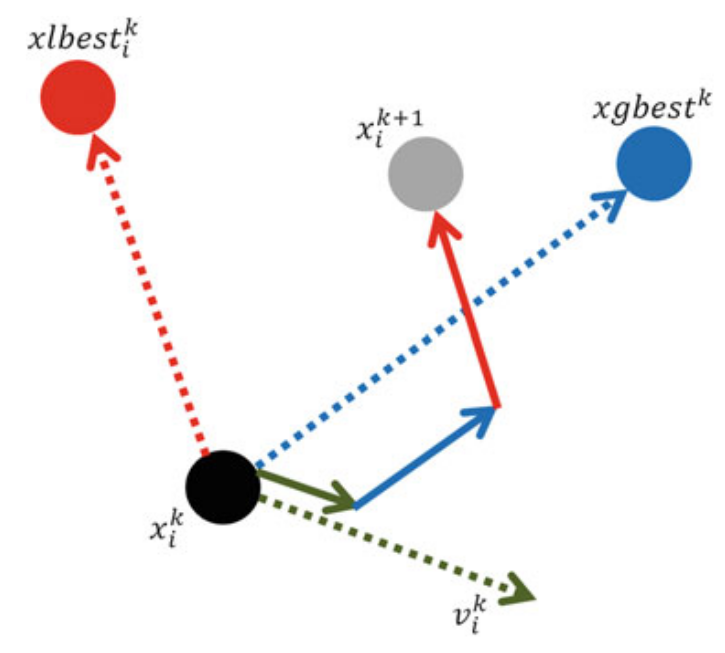
\includegraphics[height=50mm]{figures/move_particle.png} 
    \caption{Movimiento de una partícula}
    \vspace{-.25cm} 
    \caption*{Creado por Kaveh\cite{Psoexplain14}.}
    \label{fig:move_part}
\end{figure}
El modelo clásico presentado tiene ciertas complicaciones en la forma en que se actualiza la velocidad, una de ellas es la incidencia de la velocidad previa en una partícula, por lo que a modo de balancear esta variable, se añade un factor que escala esta velocidad, dado que como se explica en Kaveh \cite{Psoexplain14}, si la velocidad previa se elimina, las partículas quedan atrapadas en una región local, pero si se le da demasiado peso, converge rápidamente a un óptimo conocido. Por esto, la forma del PSO base actual, tiene un parámetro $w$, que representa la incidencia de la velocidad previa (factor de inercia). Por lo tanto, ahora se tiene que la partícula actualiza su velocidad de la siguiente forma: 
\begin{align}\label{eq:PSO}
    v_{i,j}^{k+1} &= wv_{i,j}^{k} + c_{1}r_{1}(xbest_{i,j}^k - x_{i,j}^k) + c_{2}r_{2}(xgbest_{j}^{k} - x_{i,j}^k)\\
    x_{i,j}^{k+1} &= x_{i,j}^{k} + v_{i,j}^{k+1}
\end{align}    
Donde $w$ es el factor conocido como ``inercia'' de la partícula, y regula la incidencia de la velocidad previa en la actual.\\
Finalmente, en el trabajo inicialmente citado, también se puede ver una revisión completa del estado del arte del método \emph{Particle Swarm Optimization} en términos de diseño, donde se expone las distintas modificaciones y alternativas propuestas por la literatura que pretenden mejorar aspectos como:
\begin{enumerate}
    \item  Configuración de parámetros (inercia, cognitivo, social, aleatorios).
    \item  Problemas asociados a la convergencia prematura.
    \item  Estructura de algoritmo o topologías que modifican la comunicación entre partículas (o la incidencia de las soluciones globales y particulares).
    \item  Sesgos en la búsqueda por la forma de la región o por la interacción de las partículas (operadores de combinación como el promedio, que tienden a centrar la búsqueda en determinada región).
    \item  Algoritmos híbridos con PSO.
    \item  Versión discreta del PSO. 
\end{enumerate}  

\section{Velocidad del viento}
\subsection{Distribución de Weibull}
Dado un conjunto de datos de velocidad obtenidos de la medición del viento, se puede crear un histograma que represente la frecuencia de estos datos. A partir de esto, es posible generar un modelo probabilístico que explique el comportamiento de las velocidades del viento medido, ajustándose a los datos recolectados. Dicho modelo comúnmente se basa en la distribución de Weibull, la cual es ampliamente aceptada por la comunidad dedicada al estudio meteorológico, tal y como se menciona en el trabajo de Carneiro et al. \cite{Carneiro15}, Kongnam et al. \cite{Kongnam15} y Dabbaghiyan et al.\cite{Dabbaghiyan15}. En particular, en el trabajo realizado por Carneiro et al. \cite{Carneiro15}, se describe la distribución de Weibull como: 
 \begin{align}\label{eq:weibull}
     f_{weibull}(v) = \frac{k}{c} \cdot (\frac{v}{c})^{k-1} \cdot e^{-(\frac{v}{c})^ k}
 \end{align}
 Donde $k$ y $c$ son los parámetros de ajuste que representan la forma y la escala de la distribución respectivamente, y $v$ es el valor de la velocidad del viento a la que el modelo asociará una determinada frecuencia. Un ejemplo de como se transforma esta distribución se aprecia en la figura \ref{fig:weibull_fig}, en donde se ven distintas curvas de Weibull, con diferentes parámetros $k$, y $c$ constante.
\begin{figure}[h!]
    \centering    
    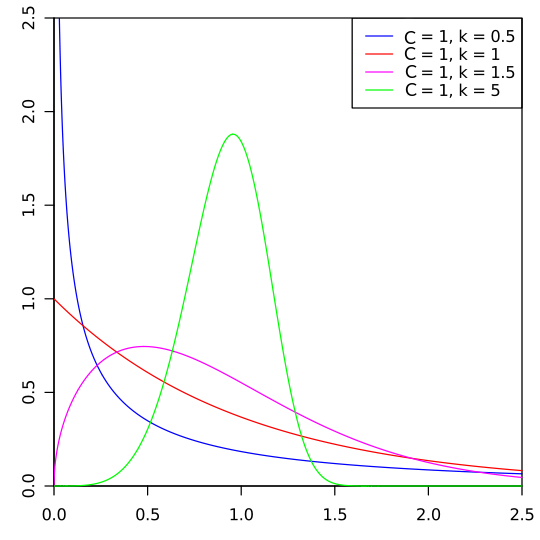
\includegraphics[height=50mm]{figures/weibull_distribution.png} 
    \caption{Función de distribución de probabilidad de Weibull}
    \vspace{-.25cm} 
    \caption*{Adaptación propia desde \cite{wikiWeibull}.}
    \label{fig:weibull_fig}
\end{figure}
 \subsection{Métodos numéricos}
 Tradicionalmente, se utilizan métodos numéricos para estimar los parámetros de la distribución de Weibull. En el artículo de Chang \cite{Chang10}, se realiza una comparación de seis métodos numéricos comúnmente utilizados para la obtención de $k$ y $c$. A continuación, se describen brevemente estos métodos:
 \begin{enumerate}
     \item \textbf{The Moment}: Se basa en la iteración numérica de las siguientes dos ecuaciones:
        \begin{align}
            \bar{v} &= c\Gamma(1 + \frac{1}{k})\\
            \sigma &= c[\Gamma(1 + \frac{2}{k}) - \Gamma^2(1 + \frac{1}{k})]^{\frac{1}{2}}
        \end{align}    
        Donde $\bar{v}$ es el promedio y $\sigma$ la desviación estándar de los datos de velocidad del viento.
    \item \textbf{Empirical}: Considerado un caso especial del método del momento. Los parámetros son calculados de la siguiente forma: 
        \begin{align}
            k &= (\frac{\sigma}{\bar{v}})^{-1.086}\\
            c &= \frac{\bar{v}}{\Gamma(1 + \frac{1}{k})}
        \end{align}    
    \item \textbf{Graphical}: Se ajustan rectas a los datos de velocidad del viento usando mínimos cuadrados. Con una doble transformación logarítmica, la función de distribución acumulativa queda:
        \begin{align}
            \ln\{-\ln[1- F(v)]\} = k\ln(v) - k\ln(c)
        \end{align}    
         Realizando un gráfico para $ln(v)$ en vez de $ln(-ln(1-F(v)))$, la pendiente de la recta que se ajusta mejor a los pares de datos es el parámetro de la forma de la distribución de Weibull. El parámetro de escala se obtiene por la intersección con la coordenada $y$.  
    \item \textbf{Maximum likelihood}: En este métodos, son necesarias muchas iteraciones. Los parámetros de Weibull están dado por:
        \begin{align}
            k &= [\frac{\sum_{i=1}^n v_i^k \ln(v_i)}{\sum_{i=1}^n v_i^k} - \frac{\sum_{i=1}^n \ln(v_i)}{n}]^{(-1)}\\
            c &= (\frac{1}{n}\sum_{i=1}^n v_i^k)^{\frac{1}{k}}
        \end{align}    
         Donde $v_i$ es la velocidad del viento en el paso $i$ y $n$ es el número de puntos de datos distintos de cero. 
    \item \textbf{Modified maximum likelihood}: Este método es utilizado si es que se tiene disponible los datos de velocidad del viento en una distribución de frecuencias. Los parámetros de Weibull son calculados como:
        \begin{align}
            k &= [\frac{\sum_{i=1}^n v_i^k \ln(v_i)f(v_i)}{\sum_{i=1}^n v_i^kf(v_I)} - \frac{\sum_{i=1}^n\ln(v_i)f(v_i)}{f(v \geq 0)}]^{-1}\\
            c &= [\frac{1}{f(v \geq 0)}\sum_{i=1}^n v_i^{k}f(v_i)]^{1/k}
        \end{align}
         Donde $v_i$ es la velocidad del viento central al intervalo $i$, $n$ es el número de intervalos. $f(v_i)$ es la frecuencia de la velocidad del viento dentro del intervalo $i$ y $f(v \geq 0)$ la probabilidad de que la velocidad del viento sea mayor o igual a cero.
    \item \textbf{Energy pattern factor method}: El factor del patrón de energía es definido como:
        \begin{align}
            E_{pf} = \frac{\bar{v^3}}{\bar{v}^3}
        \end{align}   
         Donde $\bar{v^3}$ es el promedio de las velocidades del viento cúbicas. Los parámetros de Weibull pueden ser calculados como:
        \begin{align}
            k &= 1 + \frac{3.69}{E_{pf}^2}\\
            c &= \frac{\bar{v}}{\Gamma(1 + \frac{1}{k})}
        \end{align}    
 \end{enumerate}     
 Estos métodos fueron comparados a través de pruebas de desempeño, con una simulación de Monte Carlo para este caso, y el análisis de los datos del viento con criterios tales como el test Kolmogorov-Smirnov, \emph{parameter error}, \emph{root mean square error} y el error de energía del viento. De ello, bajo distintas condiciones ciertos métodos se comportan mejor que otros ajustando la distribución de Weibull a los datos de prueba. Sin embargo, como se verá a continuación, una propuesta realizada para mejorar el ajuste a través del uso de la meta-heurística \emph{Particle Swarm Optimization}, mejora la calidad de los resultados comparado con estos métodos numéricos presentados.  
 \subsection{Particle Swarm Optimization}
 En Carneiro et al. \cite{Carneiro15}, se realiza un caso de estudio de las características del viento en las zonas costeras de Parnaiba y Maracanaú, y en una zona interior, Petrolina, en Brasil. Allí se explica la necesidad de obtener un modelo para el comportamiento estocástico del viento, de manera de poder evaluar el potencial energético de aquellas regiones. Como se menciona anteriormente, el modelo utilizado es la distribución de Weibull. Para ello, es preciso ajustar el modelo a los datos recolectados. Por esto, en el estudio mencionado, se propone un PSO para encontrar los parámetros $k$ y $c$ de la distribución de Weibull y a su vez mejorar la calidad de la solución comparada con los métodos numéricos tradicionales. Así, para lograr el objetivo, la función de aptitud se define como:
\begin{align}\label{eq:PSO_FO}
    \epsilon(v_i) = \frac{1}{2}\sum_{i=0}^{n}(f_{real}(v_i) - f_{weibull}(v_i))^2
\end{align}
Donde $\epsilon$, es el error cuadrático a minimizar entre los valores del histograma de datos y la función de distribución de Weibull.\\
El PSO utilizado es el modelo clásico presentado en la sección anterior, considerando los parámetros $w, c1$ y $c2$, sin embargo, para abolir la convergencia prematura, se establece que estos parámetros varíen durante la ejecución del algoritmo dentro de un rango definido ($w \in \{0.4, 0.9\}, c1$ y $c2 \in \{0, 2.5\}$), en donde se privilegia la exploración en el inicio de las iteraciones, para posteriormente favorecer la explotación al final de la ejecución.\\
Finalmente, para evaluar los resultados de la propuesta, se compara con el PSO con cinco de los seis métodos numéricos mencionados anteriormente utilizados para la estimación de los parámetros de Weibull: \emph{Moment Method} (M), \emph{Energy Method} (E), \emph{Energy Pattern Factor Method} (EPF), \emph{Energy Equivalent Method} (EE) y \emph{Maximum Likelihood} (ML). Además, para evaluar la eficiencia de los métodos, se utilizan tres \emph{test} estadísticos: \emph{correlation} (r), \emph{relative bias} (RB) y \emph{root mean square error} (RMSE).\\
Los resultados que se exponen en el trabajo citado son alentadores, demostrando que el PSO obtiene los mejores resultados de ajuste a los datos. Un ejemplo de esto es expuesto en la figura \ref{fig:pso_fit}.
\begin{figure}[h!]
    \centering    
    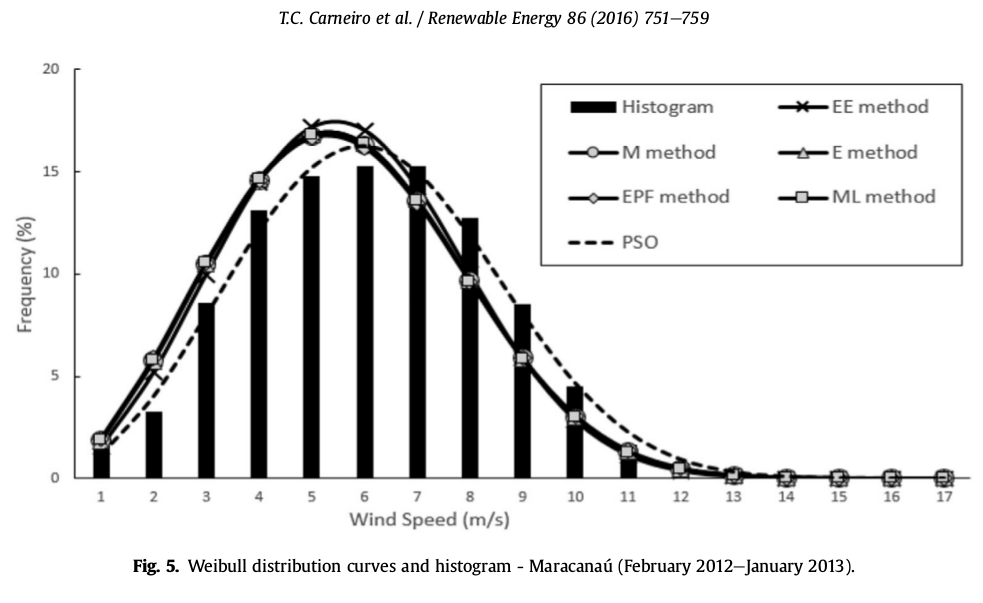
\includegraphics[height=50mm]{figures/pso_fit.png} 
    \caption{Distribución de Weibull con histograma - Maracanaú}
    \vspace{-.25cm} 
    \caption*{Creado por Carneiro et al.\cite{Carneiro15}.}
    \label{fig:pso_fit}
\end{figure}
En Kongnam et al. \cite{Kongnam15}, el PSO es utilizado para el problema del control de la velocidad de las turbinas de viento para maximizar la generación de energía. En este trabajo, se utiliza la distribución de Weibull para el modelado de la velocidad del viento. La construcción del PSO es llevada a cabo considerando el problema de la convergencia prematura, por lo que se desarrollan funciones que varían estos parámetros a lo largo de la ejecución.\\

\section{Dirección del viento}
La dirección del viento es información esencial para la investigación acerca de la energía eólica, dado que con esta, por ejemplo, se pueden ubicar de forma estratégica las turbinas que capturan la energía. En el resumen acerca de las energías renovables y sustentables\cite{Winddirelse15}, se explica que para identificar la dirección dominante del viento la función de densidad \emph{finite von Mises-Fisher} (FVMF) es utilizada para ajustarse a los datos. Para las pruebas, estos datos fueron obtenidos de cinco estaciones ubicadas en distintas zonas en la península de Malasia. La FVMF, de forma genérica, está definida de la siguiente forma:
\begin{align}
    f(x;\mu_{h}, k_{h}) = \sum_{h=1}^{H}(w_{h})\frac{k^{\frac{d}{2} - 1}}{(2\pi)^{\frac{d}{2}}I_{\frac{d}{2} - 1} (k)}e^{(k_h\mu_{h}^{T}x)}
\end{align}    
Donde $x=[cos(\theta_i), sin(\theta_i)]$, $\frac{k^{\frac{d}{2} - 1}}{(2\pi)^{\frac{d}{2}}I_{\frac{d}{2} - 1} (k)}$ es una constante de normalización, $d$ es la dimensión del vector aleatorio $x$ ($d = 2$, para este caso), $\mu_{h}$ y $k_h$ son el promedio direccional, parámetro de concentración para cada $h = 1, 2,...,H$ componente del FVFM y $w_h$ es el parámetro de mezcla (\emph{mixture parameter}).\\
Además, el parámetro de mezcla del FVMF está sujeto a la siguiente restricción:
\begin{align}
    0 \leq w_h \leq 1 \text{ y } \sum_{h=1}^{H} w_{h} = 1 \text{ para } (h=1,2,...,H) 
\end{align}
Para estimar los parámetros del FVMF, se sugiere utilizar el método \emph{expectation maximization}, debido a que los métodos regulares son incapaces de manejar la complejidad del modelo, consideraciones que se mencionan en el trabajo de Banerjee et al.\cite{Banerjee05}.\\
Por último, los resultados de este trabajo muestran que FVMF provee un razonable ajuste a diferentes conjunto de datos, obteniendo un modelo que explica más del $90\%$ de la variación de los datos, en este caso, obtenidos de estaciones ubicadas en la península de Malasia. En la figura \ref{fig:wind_dir_vonMises} se aprecia el ajuste del modelo a los datos, tanto la comparación con el histograma, como en su versión circular.\\
\begin{figure}[h!]
    \centering    
    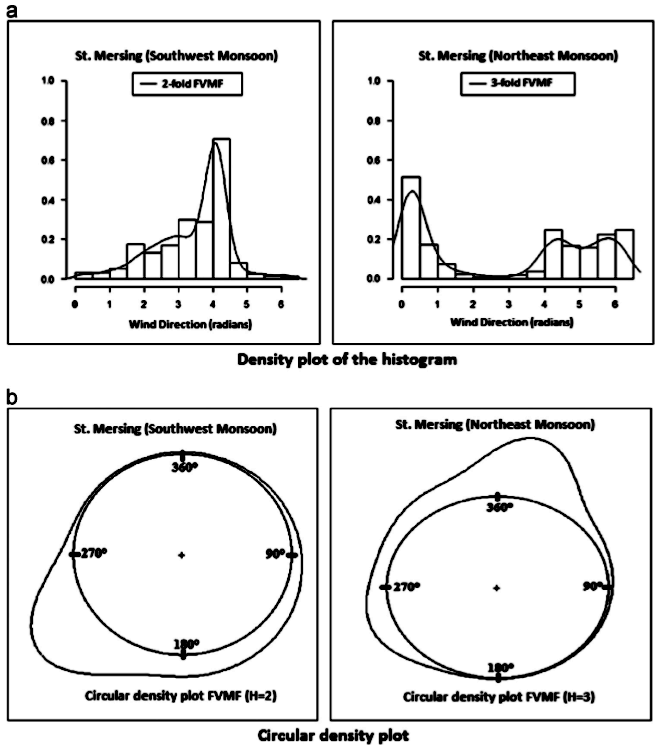
\includegraphics[height=100mm]{figures/wind_dir_vonMises.png} 
    \caption{Modelo de ajuste FVMV para suroeste y noreste en la estación Mersing}
    \vspace{-.25cm} 
    \caption*{Creado por \cite{Winddirelse15}.}
    \label{fig:wind_dir_vonMises}
\end{figure}

En el trabajo de Heckenbergerova et al.\cite{Heckenbergerova15}, se utiliza una estrategia diferente a la anteriormente mencionada. Basados en la ya mencionada meta-heurística inspirada en la biología, \emph{Particle Swarm Optimization}, proponen una forma distinta para encontrar un modelo de ajuste, utilizando la distribución estadística \emph{finite mixture of circular normal von Mises} (MvM), similar a la mencionada previamente.\\ 
En este caso, se define la distribución simple de \emph{von Mises} (SvM) como:
\begin{align}
    f(\theta; \mu, k) = \frac{1}{2{\pi}I_{0}(k)}e^{k cos(\theta - \mu)}
\end{align}    
Donde $k \geq 0$, $0 \leq \mu \leq 2\pi$, $0 \leq \theta \leq 2\pi$ y $I_0(k)$ representa la versión modificada de la función de Bessel de primera clase y orden cero:
\begin{align}
    I_0(k) = \frac{1}{\sqrt{2\pi}}\int_0^{2\pi} e^{k cos(\theta)} d\theta = \sum_{k=0}^{\infty} \frac{1}{(k!)^2}(\frac{k}{2})^{2k}
\end{align}    
Para $k=0$, la distribución SvM se vuelve uniforme alrededor de un círculo con todas las direcciones equi-probables. Cuando una colección de datos tiene más de una dirección predominante, es necesario utilizar una mezcla (\emph{mixture}) de distribuciones.
Así, la función de densidad de probabilidad \emph{finite mixture of simple von Mises} (MvM-pdf) queda como:
\begin{align}
    \phi(\theta; v) = \sum_{j=1}^{k} w_j \cdot f_j(\theta; \mu_j, k_j)
\end{align}    
Donde $k$ es el número de funciones de la mezcla, $j$ es el índice de una particular SvM-pdf con parámetros $\mu_j$ y $k_j$, $\theta$ es una variable angular ($0 \leq \theta \leq 2\pi$), y $v$ es un vector parámetro de la forma:
 \begin{align}\label{eq:sol_pso}
    v = (\mu, k, w) = (\mu_1, ..., \mu_k,k_1,...,k_k,w_1,...,w_k)
\end{align}
Para lograr el objetivo, se obtiene en primer lugar una aproximación numérica de los parámetros del MvM a partir de los datos recolectados de la dirección del viento, estrategia nombrada como estimación analítica en el trabajo de Heckenbergerova et al., para luego optimizarlos mediante el uso de un PSO, en su versión modificada, para evitar la convergencia prematura, en donde la solución está representada por una codificación del vector $\vec{v}$ mencionado anteriormente\ref{eq:sol_pso}.\\ 
Como test estadístico, es utilizado el \emph{Pearson's chi-squared goodness-off-fit}. Los resultados muestran la mejora que se logra a la estimación inicial, comparándose además con algoritmos genéticos. Sin embargo, estos no consiguen pasar el test estadístico impuesto, por lo que existe trabajo futuro  a realizar para mejorar la propuesta y lograr la precisión deseada.\\
Los resultados obtenidos para los datos recolectados en el aeropuerto de St John localizado en Newfoundland, Canadá, son apreciables en la figura \ref{fig:dir_pso}.
\begin{figure}[h!]
    \centering    
    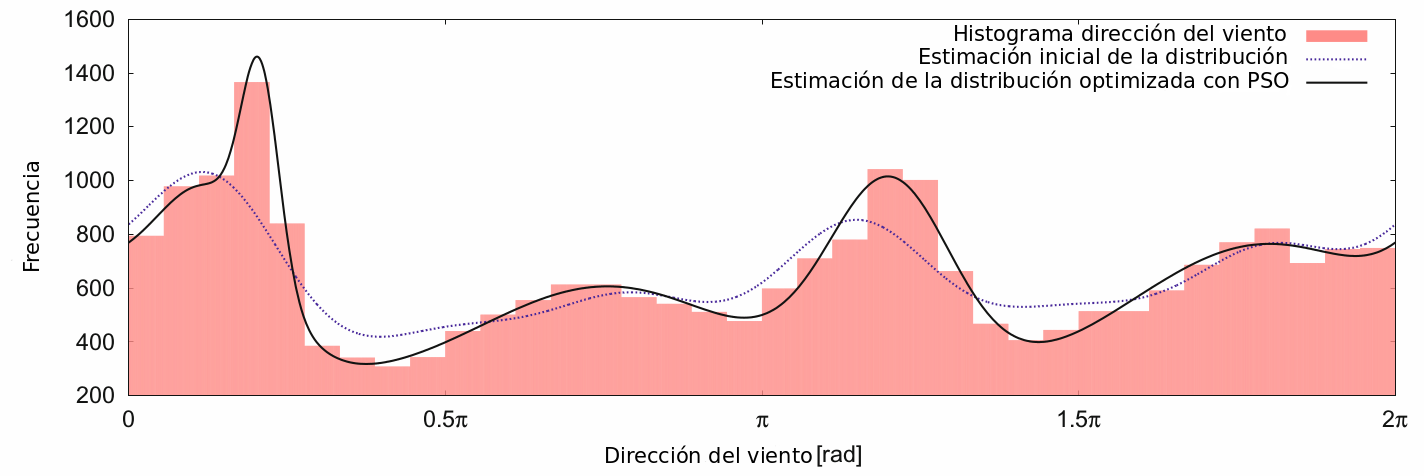
\includegraphics[height=50mm]{figures/dir_pso.png} 
    \caption{Ajuste dirección del viento, aeropuerto St. John}
    \vspace{-.25cm} 
    \caption*{Creado por Heckenbergerova et al.\cite{Heckenbergerova15}.}
    \label{fig:dir_pso}
\end{figure}


%% Desarrollo PSO velocidad

\chapter{PSO para la velocidad del viento en Valparaíso}
En este capítulo se presenta la implementación de la técnica \emph{Particle Swarm Optimization} basada principalmente en el trabajo de Carneiro et al. \cite{Carneiro15}. En principio se definen y explican los principales conceptos para entender la solución propuesta, para luego mostrar los resultados obtenidos al buscar los parámetros de ajuste de la distribución de Weibull.

\section{Modelo Matemático} \label{ss:Modelo_Mat}
Como se mencionó anteriormente, para encontrar los parámetros de la distribución de Weibull que se ajusten a los datos de prueba se utilizará la meta-heurística \emph{Particle Swarm Optimization}. La función de distribución de Weibull está definida en la ecuación \ref{eq:weibull}. La función objetivo se describe con la fórmula \ref{eq:PSO_FO} y es aquella con la que se busca minimizar el error cuadrático entre la frecuencia real de los datos y la estimada por la distribución de Weibull. Los parámetros a encontrar $k$ y $c$ deben ser $\geq 0$. Para encontrar estos parámetros se construyó el PSO que se detalla a continuación.

\section{Estructura del PSO}
Es esta sección se detallará cada una de los componentes del algoritmo, destacando algunas consideraciones importantes para el correcto desempeño de este método.
\subsection{Representación}
Cada vector posición de las partículas del enjambre representa una solución candidata la cual varía dentro de cierto espacio de búsqueda definido por los límites de las componentes. Así, para el caso de los parámetros de la distribución de Weibull, la posición de las partículas está representada por los parámetros $k$ y $c$ quedando de la forma:
\begin{align}
    x = (k, c)
\end{align}    
Para ambos parámetros, se establecen los límites entre $0 \leq (k,c) \leq 20$, criterio que se basa en el trabajo de Carneiro et al. \cite{Carneiro15}. De esta forma, las partículas se moverán dentro de ese rango, manteniéndose en los lugares que minimizan la función objetivo, la cual representa el error de la predicción de Weibull versus los datos reales.\\
Así, para cada partícula se define una estructura que posee las siguientes propiedades: 
\begin{enumerate}\label{rep:Particle}
    \item Posición: vector de largo dos de números flotantes, los cuales representan la ubicación de la partícula dentro del espacio de búsqueda y sus componentes a los parámetros $k$ y $c$.
    \item Velocidad: vector de números flotantes que representan el cambio de valor de cada componente de la posición de la partícula en determinada iteración. Se actualiza en base a la ecuación de velocidad del PSO:
    \begin{align}\label{eq:PSO}
      v_{i,j}^{k+1} &= wv_{i,j}^{k} + c_{1}r_{1}(xbest_{i,j}^k - x_{i,j}^k) + c_{2}r_{2}(xgbest_{j}^{k} - x_{i,j}^k)
    \end{align} 
    En donde $v_{i,j}^{k+1}$ es la velocidad de la partícula en el instante $k+1$, $w$, $c_1$ y $c_2$ son los parámetros de inercia, cognitivo y social respectivamente, $r_{1}$ y $r_{2}$ son números aleatorios entre $[0, 1]$, $xbest_{i,j}^k$ y $xgbest_{j}^{k}$ son la mejor solución de la partícula y la mejor solución del vecindario respectivamente en el instante $k$, $x_{i,j}^k$ representa la posición de la partícula, o la solución, en el instante $k$.    
    \item Mejor resultado personal: vector flotante que guarda la mejor posición conseguida por la partícula durante las iteraciones transcurridas.    
\end{enumerate}        
Mientras que el enjambre, siendo esencialmente una estructura que posee referencia a todas las partículas, queda representado de la siguiente forma:
\begin{enumerate}\label{rep:Swarm}
    \item Partículas: Arreglo de referencias a las estructuras de partículas creadas.
    \item Mejor posición global: De todos los mejores resultados de cada partícula, se almacena la mejor posición de todas. La que persiste al final del ciclo de iteraciones, es la solución final.
\end{enumerate} 

%% Ajustar para que sea coherente
\subsection{Consideración de los parámetros}
Los parámetros $w$ de inercia, $c_1$ cognitivo y $c_2$ social del PSO determinan con que peso inciden en el camino que siguen las partículas del enjambre, la velocidad anterior, la solución particular y la solución global respectivamente.\\ 
La inercia $w$ regula qué magnitud de la velocidad anterior se mantiene en la actual, así la partícula se comporta similar a un cuerpo desacelerando. En Kaveh \cite{Psoexplain14} se explica que en términos extremos, si la velocidad previa se elimina (peso nulo), las partículas no pueden salir del círculo local relativo a las soluciones iniciales, lo que sería equivalente a un procedimiento de búsqueda local.  Por el contrario, si se le da mucho peso, las partículas tendería a huir de las buenas posiciones conocidas.\\
El parámetro cognitivo $c_1$ controla la influencia de la mejor solución encontrada por la partícula misma en la velocidad actual. Si se le da un peso mayor a este valor, la partícula tenderá a explorar las zonas locales a la posición desde donde partió.\\
El parámetro social $c_2$ controla la influencia de la mejor solución global encontrada por el enjambre en la velocidad actual. Si se le da un peso mayor a este valor, la partícula tenderá a explotar las zonas locales a la posición de las solución global.\\
La convergencia prematura es un comportamiento presente en el \emph{Particle Swarm Optimization}, como se explica nuevamente en Kaveh \cite{Psoexplain14}. Esto se debe a que normalmente, las partículas se concentran en una ``nube'' local a la mejor solución global una vez que se ha avanzado ciertas iteraciones, lo que por una lado hace que el algoritmo sea más rápido que otras técnicas afines, como los algoritmos evolutivos, pero por otro impide que, a partir de cierto punto, se siga mejorando la solución. Por tanto, hay un límite óptimo para las iteraciones, ya que en cierto momento las partículas se quedarán atrapadas en un óptimo local.\\
A modo de evitar la convergencia prematura, varias técnicas han sido propuestas, las cuales se resumen en el trabajo de Kaveh \cite{Psoexplain14}. Para esta memoria, se utilizará la recomendación de Chang \cite{Chang10_2} para la variación de parámetros del enjambre:
\begin{align}\label{eq:VariationParameters}
    w(j) &= (1 - \frac{j}{iter_{max}})^{\alpha}(w_{max} - w_{min}) + w_{min}\\
    c_{1}(j) &= (1 - \frac{j}{iter_{max}})^{\beta}(c_{1max} - c_{1min}) + c_{1min}\\
    c_{2}(j) &= (1 - \frac{j}{iter_{max}})^{\gamma}(c_{2min} - c_{2max}) + c_{2max}
\end{align}    
Donde $w(j)$, $c_{1}(j)$, $c_{2}(j)$, son los parámetros de inercia, cognitivo y social en el instante $j$. Los valores para los rangos de los parámetros son $w_{max} = 0.9$ y $w_{min} = 0.4$, $c_{1max}$, $c_{2max}$ y $c_{1min}$, $c_{2min}$, 2.5 y 0 respectivamente. Los parámetros $\alpha, \beta, \gamma$ son definidos como 0.5, 1.5 y 1.0 respectivamente. La variable $iter_{max}$ es el máximo número de iteraciones. \\
Esta modificación provocará que las partículas ``frenen'' su convergencia al óptimo local, dado que en cada iteración se da menos peso a la solución global y mayor peso al óptimo de cada partícula y a la velocidad anterior.

\subsection{Descripción del algoritmo}
La lógica del algoritmo PSO (ver Algoritmo \ref{alg:pso}) se basa en mover las partículas dentro del rango definido para los componentes de la solución hasta que todas las partículas se concentren en alguna zona que represente una buena solución al problema, no necesariamente el óptimo. Lo importante en cada iteración es actualizar o mover el enjambre, revisar y guardar las mejores soluciones y actualizar los parámetros de inercia, cognitivo y social que definen las velocidades.
%!TEX root = main.tex

\begin{algorithm}[h!]
\caption{PSO para el ajuste de los parámetros de la distribución de Weibull}
\label{alg:pso}
\begin{algorithmic}
\REQUIRE Datos de frecuencias de velocidades del viento.
\ENSURE Valores para los parámetros $k$ y $c$.
\STATE enjambre = inicializar(w,c1,c2)
\FOR{$i = 1$ to $Iter_{max}$}
\FOR{Each partículas en enjambre}
    \STATE actualizarVelocidadPartícula(partícula)
    \STATE actualizarPosiciónPartícula(partítucla)
    \STATE guardarMejorResultadoPartícula(partícula)
\ENDFOR
\STATE guardarMejorResultadoGlobal(enjambre)
\STATE actualizarParámetros(enjambre)
\ENDFOR
\STATE retornarMejorResultadoGlobal(enjambre).
\end{algorithmic}
\end{algorithm}



\section{Resultados}\label{sec:Experimentos_velocidad}
En esta sección se presentan los resultados obtenidos en los experimentos realizados para el ajuste de la distribución de Weibull a diferentes conjuntos de datos del viento en Valparaíso.
\subsection{Experimentos}
Los experimentos fueron probados hasta en un máximo de 1000 iteraciones y 50 partículas, (A excepción del experimento donde se consideraron todos los promedios diarios, 2013, 2014 y 2015, en el cual, se utilizaron 200 partículas). Los parámetros de $w$, $c1$ y $c2$ fueron definidos tal y como explica en el modelo matemático, en la sección \ref{ss:Modelo_Mat}.\\
Los experimentos fueron realizados con datos del viento obtenidos por la Armada de Chile para la región de Valparaíso en los años 2013, 2014 y 2015. Estos fueron tratados mediante \emph{scripts} desarrollados en \emph{Python} para obtener las frecuencias de las distintas velocidades del viento registradas a lo largo del año. Los datos se organizaban de la siguiente forma: Por cada año, se tiene una tabla en un archivo excel de cada mes, en donde se registra por cada fila los resultados de la medición de cada día. Las mediciones son registradas en un intervalo de tres horas, es decir, se tienen registros diarios para las 3:00, 6:00, 9:00, 12:00, 15:00, 18:00, 21:00 y 00:00 horas. Un ejemplo es la tabla mostrada en la Figura \ref{fig:example_data}.\\
 \begin{figure}[h!]
    \centering
    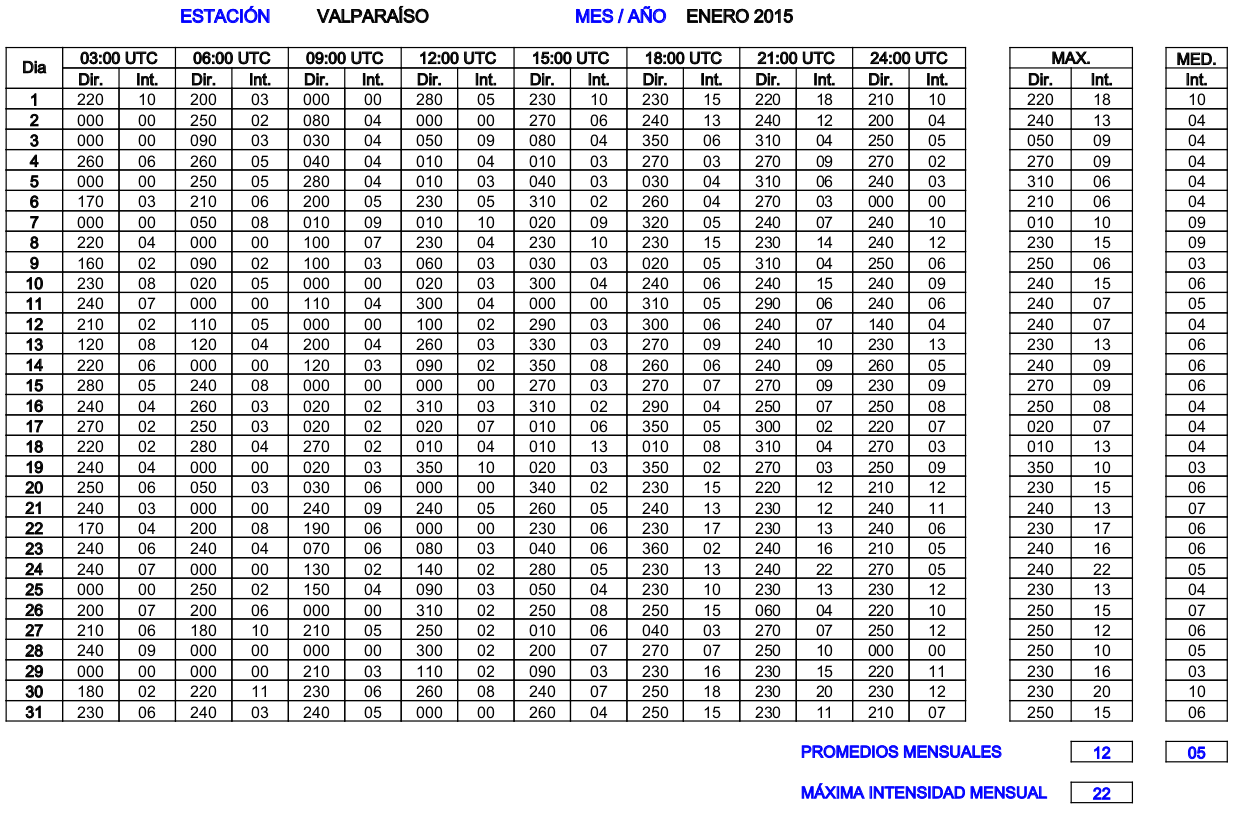
\includegraphics[height=100mm]{figures/example_data.png}
    \caption{Ejemplo colección de datos Enero Valparaíso 2015}
    \vspace{-.25cm}
    \caption*{Obtenido desde el Instituto Meteorológico de la Armada de Chile.}
    \label{fig:example_data}
 \end{figure}
El ajuste de la distribución de Weibull a estos datos de velocidad del viento se hizo considerando las siguientes configuraciones para el cálculo del
histograma de frecuencias:
\begin{enumerate}
  \item \textbf{Todos los años}. Se considera el promedio diario de velocidad del viento como dato unitario para el cálculo de las frecuencias, considerando
  todos los días en el intervalo de Enero del 2013 hasta Diciembre del 2015.
  \item \textbf{Anual}. Se considera el promedio diario de velocidad del viento como dato unitario para el cálculo de las frecuencias en
  un lapso anual (2013, 2014 y 2015).
  \item \textbf{Por temporada}. Se considera el promedio diario de velocidad del viento como dato unitario para el cálculo de las frecuencias en
  un lapso de tres meses (Enero - Marzo ; Abril - Junio; Julio - Septiembre; Octubre - Diciembre).
  \item \textbf{Datos brutos}. Se considera cada medición realizada (8 por día) como dato unitario, en un lapso de un año.
\end{enumerate}

Una vez obtenido los datos de frecuencias, se procede a aplicar el algoritmo \emph{Particle Swarm Optimization} donde se obtienen los parámetros de ajuste $k$ y $c$. De esta manera, se evalúa la calidad del modelo generado (distribución de densidad de probabilidad de Weibull), para las distintas configuraciones mediante gráficos y los siguientes test estadísticos (utilizados también en el trabajo de Carneiro et al. \cite{Carneiro15}):
\begin{enumerate}
    \item \emph{Root Mean Square Error}
        \begin{align}
            RMSE = \sqrt{\frac{\sum_{i=1}^{N}(X_i - Y_i)^2}{N}}
        \end{align}    
    \item \emph{Correlation}
        \begin{align}
            r = \frac{\sum_{i=1}^{N}(X_i - X_{med})\cdot(Y_i - Y_{med})}{\sqrt{\sum_{i=1}^{N}(X_i - X_{med})^2}\cdot\sqrt{\sum_{i=1}^{N}(Y_i - Y_{med})^2}}
        \end{align}    
    \item \emph{Relative Bias}
        \begin{align}
            RB = \frac{X_{med} - Y_{med}}{Y_{med}}  
        \end{align}    
\end{enumerate}        
Donde $N$ es el número de datos, $Y_i$ la frecuencia de dichos datos, $X_i$ la frecuencia entregada por la distribución de Weibull, $X_{med}$ la media de $X_i$ e $Y_{med}$ la media de $Y_i$. \\

Las pruebas fueron realizadas en un computador con sistema operativo Ubuntu 16.04 64-bit, 3.8 GB de memoria y procesador doble núcleo Intel Pentium 2.60 GHz. 

\subsection{Análisis de los resultados}
\subsubsection{Visualización de los datos}
Los gráficos \ref{fig:data_valpo_13}, \ref{fig:data_valpo_14} y \ref{fig:data_valpo_15} muestran la distribución de datos de velocidad del viento en Valparaíso a lo largo de los meses del año y las horas del día, lo cual permite visualizar la naturaleza de la intensidad del viento de forma cualitativa.
Por ejemplo, se logra apreciar que las máximas velocidades son obtenidas en los meses finales de primavera y comienzos de verano.\\
Las superficies que se exponen no representan la distribución continua de los datos. Estos fueron graficados de forma discreta y posteriormente la herramienta utilizada para generar la superficie unió los puntos mediante rectas.\\
\begin{figure}[ht!]
     \centering
     \captionsetup{justification=centering,margin=2cm}
        \subfigure[Vientos Valparaíso 2013.]{
            \label{fig:data_valpo_13}
            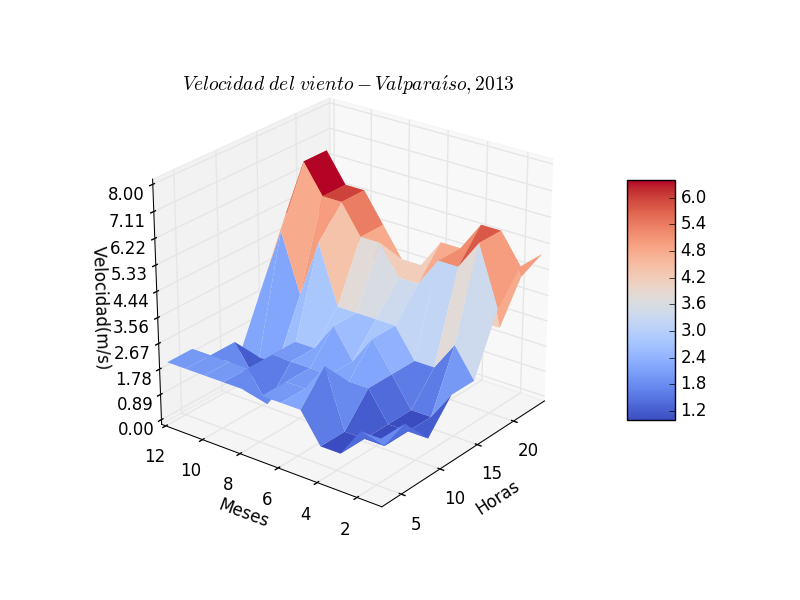
\includegraphics[width=0.45\textwidth]{figures/3d_data_2013.png}
        }%
         \subfigure[Vientos Valparaíso 2014.]{
            \label{fig:data_valpo_14}
            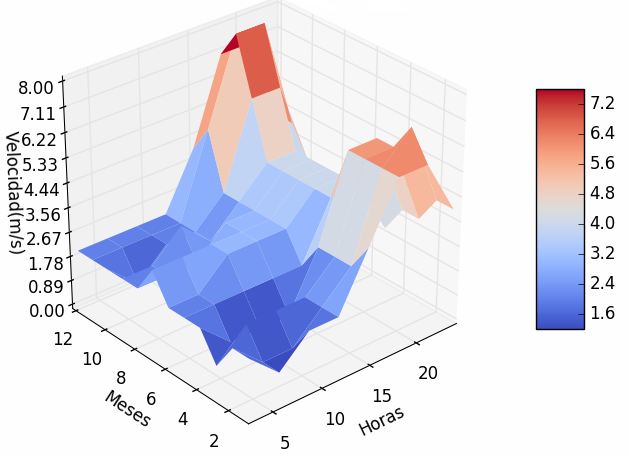
\includegraphics[width=0.45\textwidth]{figures/3d_data_2014.png}
        }\\
         \subfigure[Vientos Valparaíso 2015.]{
            \label{fig:data_valpo_15}
            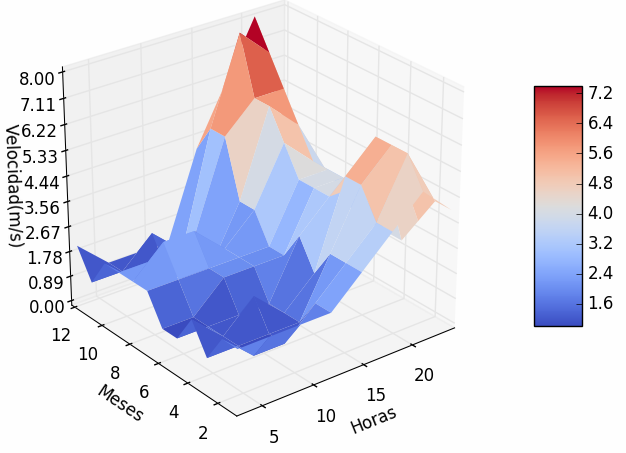
\includegraphics[width=0.45\textwidth]{figures/3d_data_2015.png}
        }%
    \caption{Superficie de datos viento de Valparaíso.\\ Fuente: Elaboración Propia.}
    \label{fig:subfigures}
\end{figure}

\subsubsection{Experimento 1, datos anuales y promedios diarios}
Las figuras \ref{fig:pso_valpo_13}, \ref{fig:pso_valpo_14} y \ref{fig:pso_valpo_15} muestran el ajuste de la distribución de Weibull a los histogramas de datos del viento (promedios diarios), con los parámetros $k$ y $c$  que se muestran en las primeras tres filas de la tabla \ref{table:stadistical_tests} determinados por el PSO. El ajuste tiene buena forma, lo cual es corroborado por los datos estadísticos obtenidos con los test previamente mencionados (RMSE, r, RB), expuestos en la tabla \ref{table:stadistical_tests} en las filas 1, 2 y 3. Si se compara con la precisión conseguida en el trabajo de Carneiro et al. \cite{Carneiro15}, se aprecia que el ajuste conseguido es levemente más impreciso, sobre todo en lo relativo al test \emph{relative bias} (RB) el cual es una medida de distancia de la frecuencia estimada con la de los datos. Esto podría deberse a la naturaleza de los datos 
trabajados.\\
\begin{figure}[ht!]
    \centering
    \captionsetup{justification=centering,margin=2cm}
        \subfigure[PSO Valparaíso 2013.]{
            \label{fig:pso_valpo_13}
            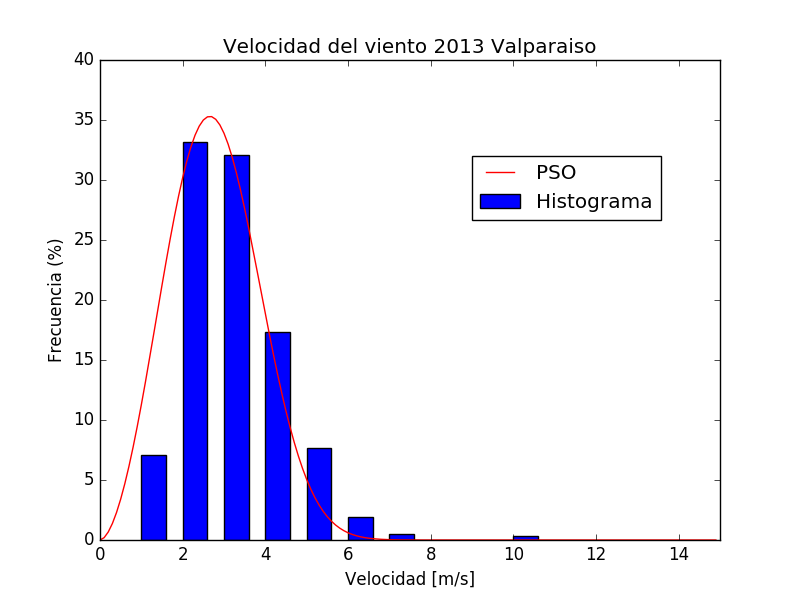
\includegraphics[width=0.45\textwidth]{figures/result_2013.png}
        }%
        \subfigure[PSO Valparaíso 2014.]{
            \label{fig:pso_valpo_14}
            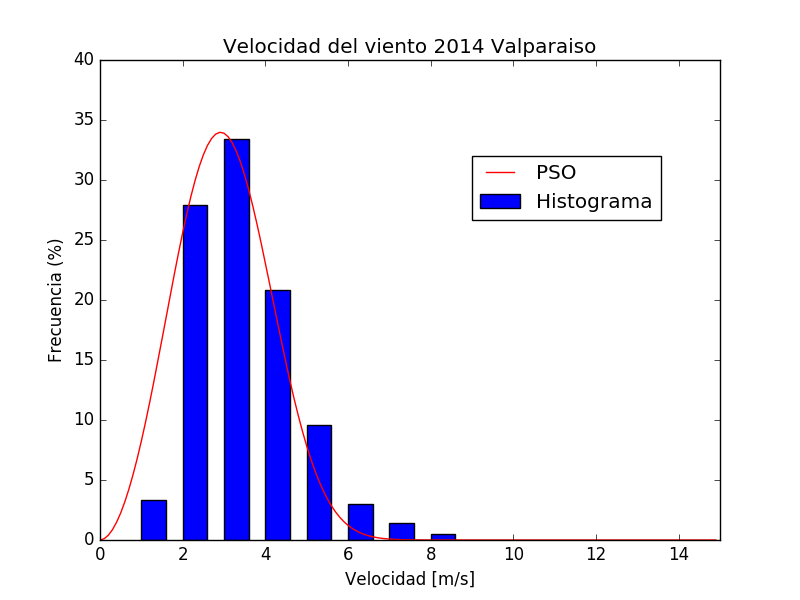
\includegraphics[width=0.45\textwidth]{figures/result_2014.png}
        }\\
        \subfigure[PSO Valparaíso 2015.]{
            \label{fig:pso_valpo_15}
            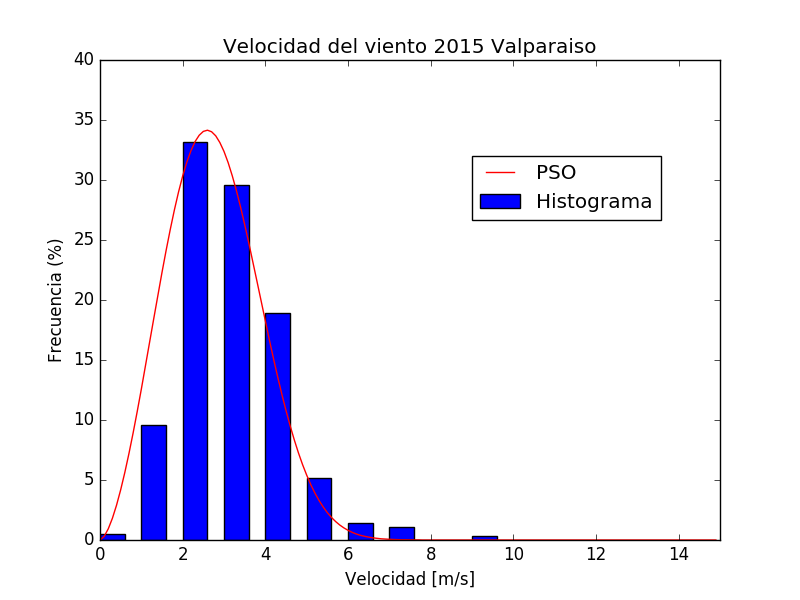
\includegraphics[width=0.45\textwidth]{figures/result_2015.png}
        }%
    \caption{Ajuste con PSO a datos del viento de Valparaíso.\\ Fuente: Elaboración Propia.}
    \label{fig:subfigures}
\end{figure}

\subsubsection{Experimento 2, datos de tres años y promedios diarios}
En este experimento se realizó el ajuste considerando los promedios diarios y un intervalo de tres años consecutivos. El gráfico \ref{fig:pso_valpo_15_14_13_lq}, muestra el resultado del ajuste con PSO y la configuración estándar de los demás experimentos, es decir, 100 iteraciones y 50 partículas. En este gráfico se aprecia que el ajuste no es bueno, a pesar de las cifras en la tabla \ref{table:stadistical_tests}, fila 4: PSO (50p), dado que oscila bastante alrededor de las barras del histograma, por lo que se repite el experimento aumentando el número de partículas a 200 obteniendo el gráfico \ref{fig:pso_valpo_15_14_13}, con el cual se obtiene un ajuste más adecuado, además de mejorar los resultados de los test estadísticos (tabla \ref{table:stadistical_tests}, fila 5: PSO (200p)).\\
\begin{figure}[ht!]
    \centering
    \captionsetup{justification=centering,margin=2cm}
        \subfigure[Buen ajuste PSO Valparaíso 2013.]{
            \label{fig:pso_valpo_15_14_13}
            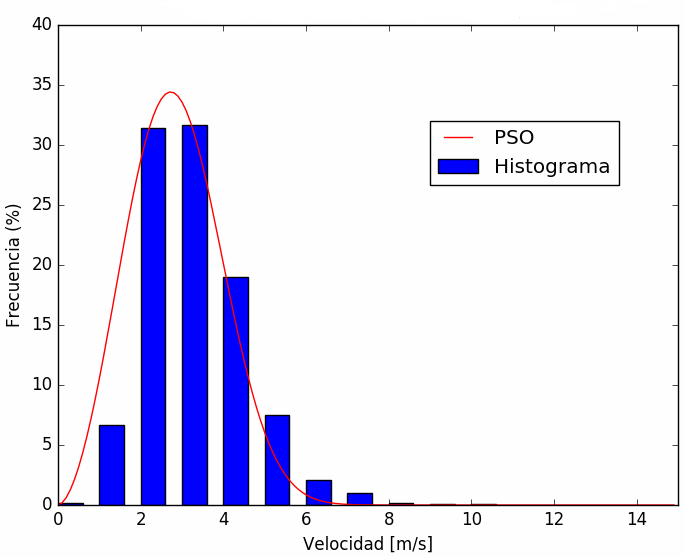
\includegraphics[width=0.45\textwidth]{figures/result_13-14-15.png}
        }%
        \subfigure[Mal ajuste PSO Valparaíso 2013.]{
            \label{fig:pso_valpo_15_14_13_lq}
            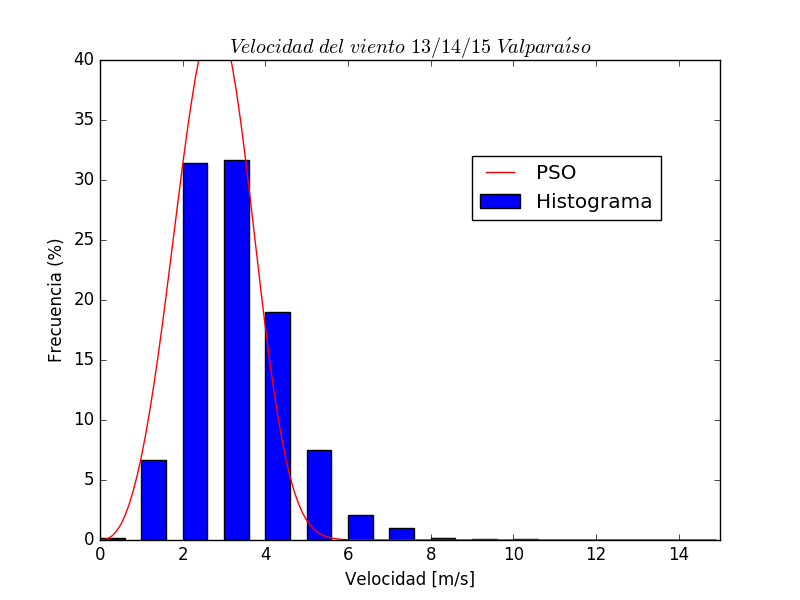
\includegraphics[width=0.45\textwidth]{figures/result_13-14-15_low_quality.png}
        }%
    \caption{Ajuste con PSO a datos Valparaíso 2015, 2014 y 2013, baja y buena calidad.\\ Fuente: Elaboración Propia.}
    \label{fig:subfigures}
\end{figure}

\subsubsection{Experimento 3, ajuste a datos anuales con resultados del experimento 2}
Los gráficos \ref{fig:pso_valpo_13_all_data}, \ref{fig:pso_valpo_14_all_data} y \ref{fig:pso_valpo_15_all_data} son ajustes de Weibull con los parámetros obtenidos en el experimento anterior. Es decir, la idea es evaluar el modelo general de los tres años versus el histograma de datos de cada año en particular.
El ajuste desde los resultados estadísticos (tabla \ref{table:stadistical_tests}), es levemente menos preciso que el modelo ajustado a cada año en particular, pero sigue siendo aceptable como posible opción a considerar.
\begin{figure}[ht!]
    \centering
    \captionsetup{justification=centering,margin=2cm}
    \subfigure[Velocidad viento Valparaíso 2013.]{
        \label{fig:pso_valpo_13_all_data}
        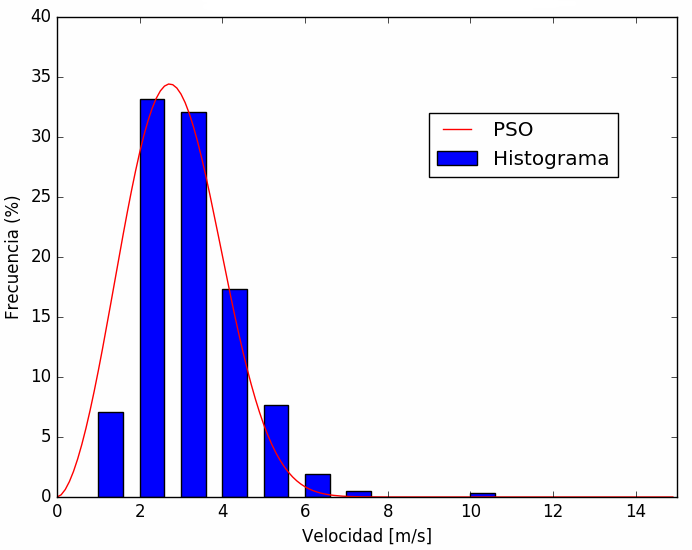
\includegraphics[width=0.45\textwidth]{figures/result_2013_fit_all_data.png}
    }%  
    \subfigure[Velocidad viento Valparaíso 2014.]{
        \label{fig:pso_valpo_14_all_data}
        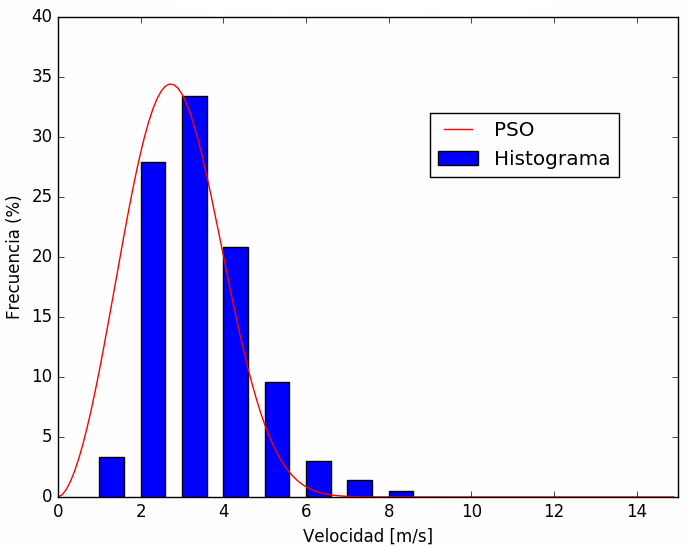
\includegraphics[width=0.45\textwidth]{figures/result_2014_fit_all_data.png}
    }\\   
    \subfigure[Velocidad viento Valparaíso 2015.]{
        \label{fig:pso_valpo_15_all_data}
        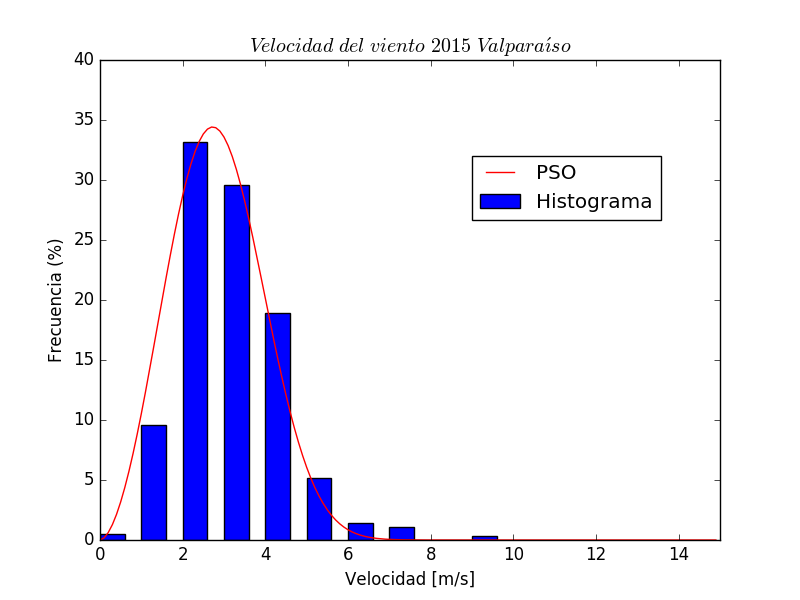
\includegraphics[width=0.45\textwidth]{figures/result_2015_fit_all_data.png}
    }%     

    \caption{Ajuste con PSO a registros del viento en Valparaíso (Con todos los datos).\\ Fuente: Elaboración Propia.}
    \label{fig:subfigures}
\end{figure}

\subsubsection{Experimento 4, ajuste a datos de tres meses y promedios diarios}
Es posible que se requiera un análisis más acotado, por ello los gráficos \ref{fig:pso_valpo_15_ene_mar}, \ref{fig:pso_valpo_15_abr_jun}, 
\ref{fig:pso_valpo_15_jul_sep}, \ref{fig:pso_valpo_15_oct_dic}, muestran un ajuste considerando un lapso de 3 meses para el año 2015, con el
que se demuestra que es posible definir cualquier intervalo (manteniendo como unidad de dato el promedio diario de velocidad del viento)
 y obtener un ajuste adecuado de los datos mediante la distribución de Weibull.

\begin{figure}[ht!]
    \centering
    \captionsetup{justification=centering,margin=2cm}
    \subfigure[Enero - Marzo.]{
        \label{fig:pso_valpo_15_ene_mar}
        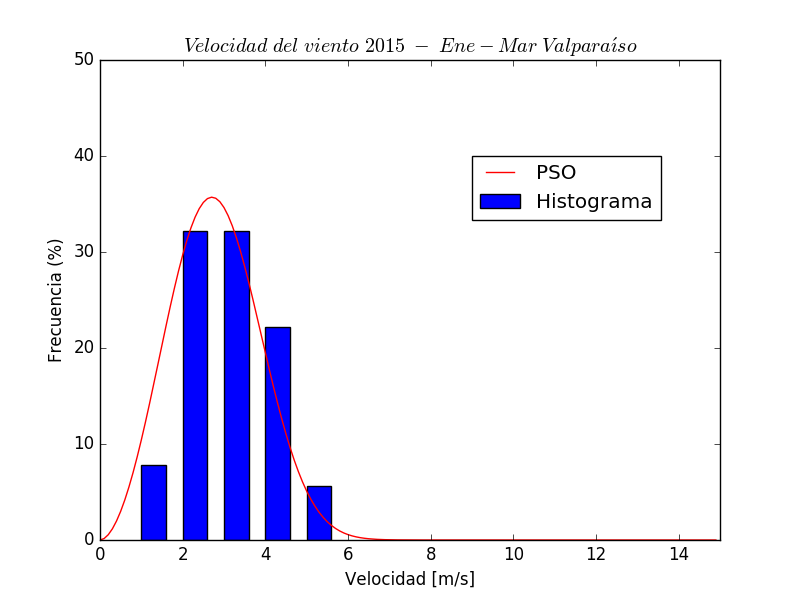
\includegraphics[width=0.45\textwidth]{figures/result_2015_Ene-Mar.png}
    }%  
    \subfigure[Abril - Junio.]{
        \label{fig:pso_valpo_15_abr_jun}
        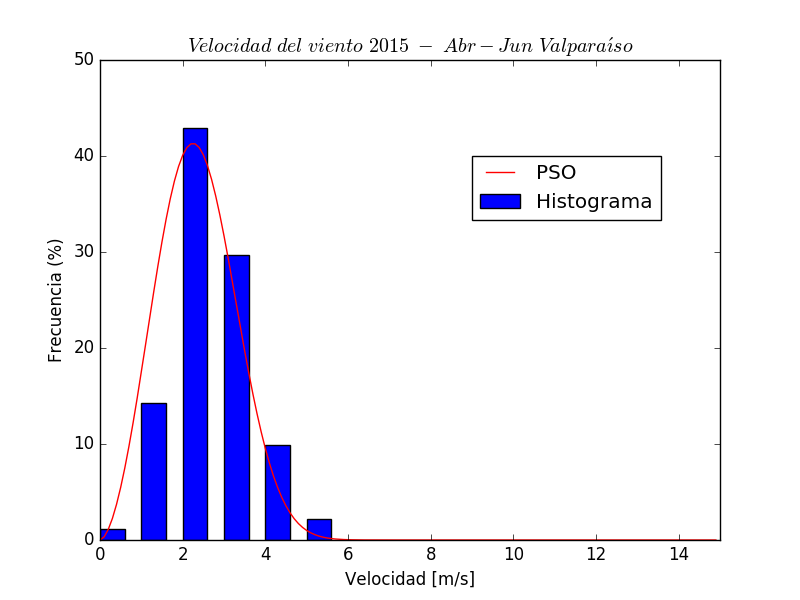
\includegraphics[width=0.45\textwidth]{figures/result_2015_Abr-Jun.png}
    }\\  
    \subfigure[Julio - Septiembre.]{
        \label{fig:pso_valpo_15_jul_sep}
        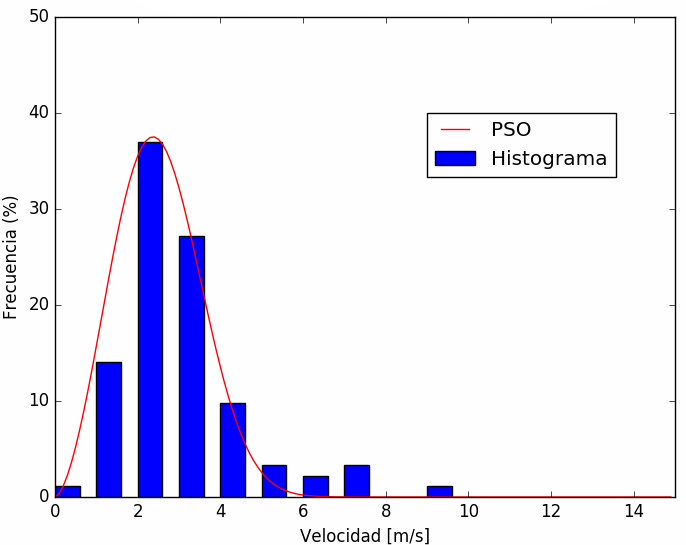
\includegraphics[width=0.45\textwidth]{figures/result_2015_Jul-Sep.png}
    }% 
    \subfigure[Octubre - Diciembre.]{
        \label{fig:pso_valpo_15_oct_dic}
        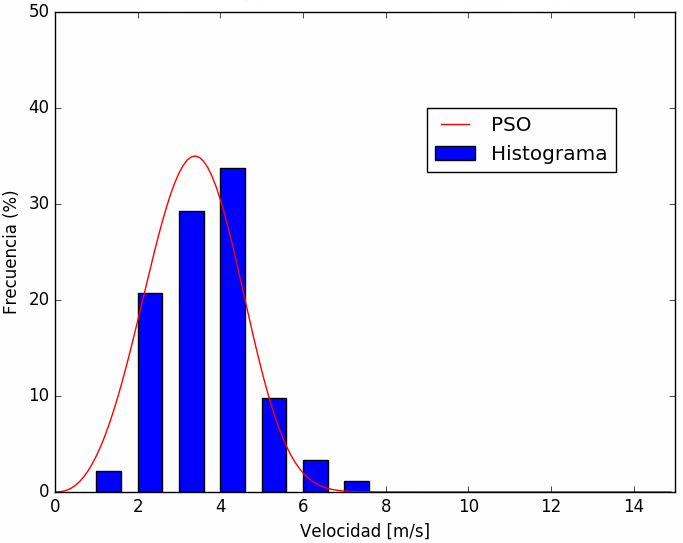
\includegraphics[width=0.45\textwidth]{figures/result_2015_Oct-Dic.png}
    }%  
    \caption{Ajuste con PSO a datos Valparaíso 2015, por rango de meses.\\ Fuente: Elaboración Propia.}
    \label{fig:subfigures}
\end{figure}

\subsubsection{Experimento 4, ajuste a datos año 2015 y datos brutos}
La razón de por qué se utiliza el promedio diario de los datos del viento para ajustar Weibull y no las mediciones puras (las mediciones tomadas cada 3 horas diariamente) es expuesta en el gráfico \ref{fig:pso_valpo_15_all_data}. La distribución de Weibull no se ajusta a una distribución de datos con más de un máximo, por lo que de requerirse un modelo para este caso se debe buscar otra distribución o modificar la distribución de Weibull. Es por ello que normalmente se utiliza un promedio de los datos, como se realiza en el trabajo de Farade \cite{Fadare08}.
\begin{figure}[ht!]
    \centering
    \captionsetup{justification=centering,margin=2cm}
    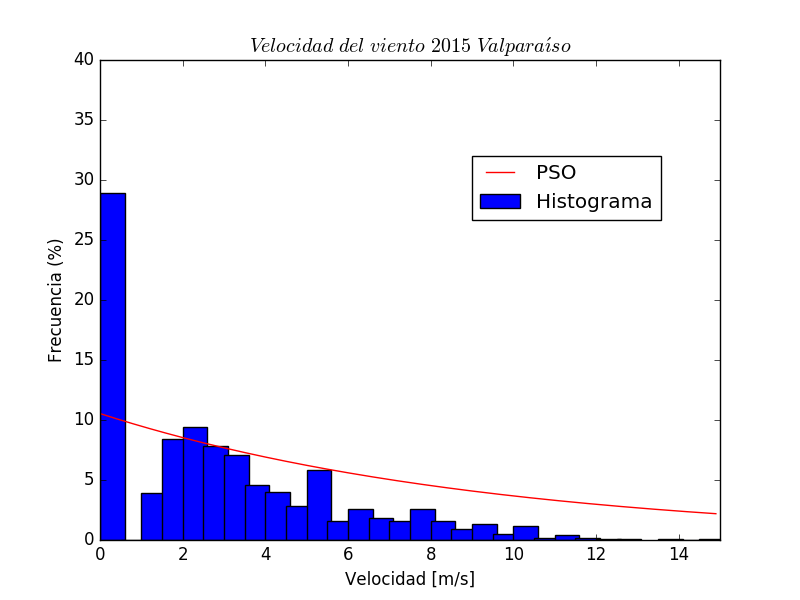
\includegraphics[width=0.45\textwidth]{figures/result_2015_all_data.png}
    \caption{Ajuste con PSO a datos (cifras puras) Valparaíso 2015, 2014, 2013}
    \vspace{-.25cm}
    \caption*{Fuente: Elaboración Propia.}
    \label{fig:pso_valpo_15_all_data}
\end{figure}
\pagebreak
\newpage
\subsubsection{Resumen de los experimentos}
En esta sección se exponen los resultados obtenidos de los experimentos realizados. En este caso la aplicación de la propuesta realizada en Carneiro et al. \cite{Carneiro15}, obtuvo los resultados esperados en cuanto a la calidad del ajuste de la distribución de Weibull a los datos del viento de Valparaíso.\\
La tabla se organiza como se explica a continuación:
\begin{enumerate}
  \item \textbf{Método}: Método utilizado para el ajuste de los parámetros de Weibull.
  \item \textbf{Periodo}: Periodo de tiempo considerado para los datos en el experimento.
  \item \textbf{k}: Parámetro $k$ de la distribución de Weibull.
  \item \textbf{c}: Parámetro $c$ de la distribución de Weibull.
  \item \textbf{RMSE}: Test estadístico conocido como \emph{root mean square error}.
  \item \textbf{r}: Test estadístico conocido como \emph{correlation}.
  \item \textbf{RB}: Test estadístico conocido como \emph{relative bias}.
  \item \textbf{Tiempo}: Tiempo total de ejecución del algoritmo.
\end{enumerate}
Los tiempos omitidos en la Tabla \ref{table:stadistical_tests}, en las filas 6, 7 y 8 indican que no se calcularon los parámetros de la función de densidad, sino que se utilizaron los obtenidos previamente, en el experimento de la fila 5. El número de iteraciones del PSO no se considera debido a que sólo se itera en la fase de desarrollo del algoritmo. Cuando este está completo, basta con una ejecución para tener el resultado definitivo del experimento.
\begin{table}[ht!]
    %\centering
    \caption{Tabla de pruebas, PSO velocidad del viento}
    \label{table:stadistical_tests}
    \resizebox{\textwidth}{!}{
    \begin{tabular}{|c|c|c|c|c|c|c|c|c|}
        \hline
        \textbf{\#} & \textbf{Método} & \textbf{Periodo} & \textbf{k} & \textbf{c} & \textbf{RMSE} & \textbf{r} & \textbf{RB} & \textbf{Tiempo}\\
        \hline
        1   & PSO                 & 2013        & 2.78 & 3.12                   & 2.26$\cdot 10^{-2}$ & 0.984  & 1.98$\cdot 10^{-3}$  & 1.74s\\
        2   & PSO                 & 2014        & 2.91 & 3.37                   & 2.32$\cdot 10^{-2}$ & 0.982  & 7.54$\cdot 10^{-4}$  & 1.63s\\
        3   & PSO                 & 2015        & 2.65 & 3.10                   & 1.64$\cdot 10^{-2}$ & 0.992  & 3.02$\cdot 10^{-3}$  & 1.59s\\
        \hline
        4   & PSO (50p)           & 2015-14-13  & 3.47 & 3.07                   & 3.61$\cdot 10^{-2}$ & 0.975  & 4.11$\cdot 10^{-3}$  & 2.00s\\
        5   & PSO (200p)          & 2015-14-13  & 2.78 & 3.20                   & 1.61$\cdot 10^{-2}$ & 0.994  & 1.91$\cdot 10^{-3}$  & 7.78s\\
        \hline
        6   & PSO (200p y todos los datos)          & 2013        & 2.78 & 3.20 & 2.41$\cdot 10^{-2}$ & 0.981  & 1.92$\cdot 10^{-3}$  & - \\
        7   & PSO (200p y todos los datos)          & 2014        & 2.78 & 3.20 & 3.01$\cdot 10^{-2}$ & 0.970  & 8.89$\cdot 10^{-6}$  & - \\
        8   & PSO (200p y todos los datos)          & 2015        & 2.78 & 3.20 & 2.02$\cdot 10^{-2}$ & 0.986  & 1.92$\cdot 10^{-3}$  & - \\
        \hline
        9   & PSO                 & Ene-Mar     & 2.85 & 3.15                   & 2.31$\cdot 10^{-2}$ & 0.982  & 6.41$\cdot 10^{-3}$  & 1.29s\\
        10  & PSO                 & Abr-Jun     & 2.76 & 2.65                   & 2.04$\cdot 10^{-2}$ & 0.993  & 3.03$\cdot 10^{-3}$  & 1.34s\\
        11  & PSO                 & Jul-Sep     & 2.66 & 2.83                   & 2.51$\cdot 10^{-2}$ & 0.985  & 4.43$\cdot 10^{-3}$  & 1.19s\\
        12  & PSO                 & Oct-Dic     & 3.40 & 3.75                   & 2.60$\cdot 10^{-2}$ & 0.978  & 7.16$\cdot 10^{-4}$  & 1.30s\\
        \hline 
        13  & PSO (datos brutos)  & 2015        & 1.00 & 9.49                   & 4.51$\cdot 10^{-2}$ & 0.751  & 6.7$\cdot 10^{-1}$   & 1.65s\\ 
        \hline
     \end{tabular}
    }   
\end{table}
        %\hline
        %\textbf{\#} & \textbf{Método} & \textbf{Periodo} & \textbf{k} & \textbf{c} & \textbf{RMSE} & \textbf{r} & \textbf{RB} & \textbf{Tiempo}\\
        %\hline
        %1   & PSO                 & 2013        & 2.78 & 3.12 & 0.0226585230791 & 0.984353070415  & 0.00197971468299  & 1.748337s\\
        %2   & PSO                 & 2014        & 2.91 & 3.37 & 0.0232779965263 & 0.982087745069  & 0.000754465101398 & 1.630882s\\
        %3   & PSO                 & 2015        & 2.65 & 3.10 & 0.0164721412159 & 0.992323803649  & 0.00302918178445  & 1.599510s\\
        %\hline
        %4   & PSO (50p)           & 2015-14-13  & 3.47 & 3.07 & 0.0360794587206 & 0.975240385258  & 0.000411212628513 & 2.002766s\\
        %5   & PSO (200p)          & 2015-14-13  & 2.78 & 3.20 & 0.016175531561  & 0.994989105807  & 0.00190916669626  & 7.781343s\\
        %\hline
        %6   & PSO (200p y todos los datos)          & 2013        & 2.78 & 3.20 & 0.0240448436122 & 0.981963054492  & 0.00192186034284  & - \\
        %7   & PSO (200p y todos los datos)          & 2014        & 2.78 & 3.20 & 0.0301463089474 & 0.970662237238  & 0.00000889024791  & - \\
        %8   & PSO (200p y todos los datos)          & 2015        & 2.78 & 3.20 & 0.0202342934641 & 0.98662798667   & 0.00192175053173  & - \\
        %\hline
        %9   & PSO                 & Ene-Mar     & 2.85 & 3.15 & 0.0230380400157 & 0.982158006469  & 0.00641888742608  & 1.293452s\\
        %10  & PSO                 & Abr-Jun     & 2.76 & 2.65 & 0.0204300909755 & 0.993857185938  & 0.00303620481316  & 1.345529s\\
        %11  & PSO                 & Jul-Sep     & 2.66 & 2.83 & 0.0251002816356 & 0.985858767021  & 0.00443453471038  & 1.1998735s\\
        %12  & PSO                 & Oct-Dic     & 3.40 & 3.75 & 0.0260278634297 & 0.978479679326  & 0.00071665352959  & 1.3032119s\\
        %\hline 
        %13  & PSO (datos brutos)  & 2015        & 1.00 & 9.49 & 0.0451794472583 & 0.751732944794  & 0.676094670465 & 1.6544219s\\ 
        %\hline
\newpage
\section{Conclusiones del capítulo}
En este capítulo se implementó la propuesta realizada en Carneiro et al. \cite{Carneiro15} para ajustar los parámetros de la distribución de Weibull a los datos de velocidad del viento en Valparaíso. Los resultados confirman que el método propuesto permite obtener soluciones de buena calidad, bajo el punto de vista de los test estadísticos aplicados (RMSE, r y RB), y los gráficos generados. Sin embargo, se debe tener en consideración que la distribución de Weibull representa el promedio diario de velocidades medidas del viento, detalle que no siempre se menciona en los trabajos que utilizan esta distribución, pero que se explican en algunos como en Fadare \cite{Fadare08}. Este modelo es útil para aplicaciones como, la estimación del potencial eléctrico en determinada región.\\
Si se desea otra representación para las velocidades del viento, que permita representar velocidades predominantes, o una descripción más directa de los datos, como los representados en la Figura \ref{fig:pso_valpo_15_all_data}, se debe buscar otra distribución o una versión modificada de Weibull.
%% Desarrollo PSO velocidad

\chapter{PSO para la dirección del viento en Valparaíso}
\section{Modelo Matemático}\label{ss:model_math_dir} 
Como se comenta anteriormente, la distribución de densidad de probabilidad que se utilizará para describir la distribución de datos de dirección del viento
es la \emph{finite mixtures of von mises distribution} descrita en \ref{eq:mixtureVonMises}, la cual consiste básicamente en una combinación lineal de la \emph{simple von Mises distribution} descrita en \ref{eq:simpleVonMises}.\\ 
De forma preliminar, los datos se ordenan en un histograma de densidad con el cual se obtiene un esqueleto de la distribución de densidad de probabilidad. Posteriormente se requieren encontrar los parámetros de ajuste $\mu_j$, $k_j$ y $w_j$ para cada $j$-ésima \emph{simple von Mises distribution}. La forma en que
se realiza esto último en este trabajo está basado en el documento de Carta et al. \cite{Carta07} y se describe a continuación.\\
Para la construcción del histograma se divide el rango de datos que va de 0 a $2\pi$ en $T$ clases con frecuencia $O_i$ la cual representa la suma de las observaciones en el rango de la clase $T$. Posteriormente se definen $k$ sectores del mismo largo desde las $T$ clases, relacionados al número de direcciones de viento predominantes (o con mayor frecuencia). Esto define el número de funciones de von Mises a utilizar. La estimación de $k$ se realiza mediante la observación del histograma de los datos, observando la cantidad de direcciones con altas frecuencias (también puede ser considerado un parámetro de ajuste, que requiera de pruebas empíricas para encontrar el valor adecuado). Además, se sigue la observación empírica en el trabajo de Carta et al. \cite{Carta07}, en donde se concluye que valores superiores a 6 \emph{mixtures} no mejoran considerablemente la calidad del ajuste.\\
Para la aproximación inicial de los parámetros de la \emph{mixture of von mises distribution} se utiliza una estimación numérica, utilizada por Heckenbergerova et al. \cite{Heckenbergerova15} \cite{Heckenbergerova13} y Carta et al. \cite{Carta07}, basada en los datos recolectados acerca de la dirección del viento.\\
Sea $j \in \{1 ... k\}$ el subíndice del sector representado por la $j$-ésima función de von Mises.\\
La dirección del viento predominante $\mu_j$ se estima de la siguiente forma:
\begin{align}\label{eq:Prevailing_Param}
    \mu_j &= 
        \left\{
            \begin{array}{ll}
                arctan(\frac{s_j}{c_j})  & s_j \geq 0, c_j > 0\\
                \frac{\pi}{2} & s_j > 0, c_j = 0\\
                \pi + arctan(\frac{s_j}{c_j}) & c_j < 0\\
                \pi & s_j > 0, c_j = -1\\
                2\pi + arctan(\frac{s_j}{c_j}) & s_j < 0, c_j > 0\\
                3\frac{\pi}{2} & s_j < 0, c_j = 0\\
            \end{array}
        \right.
\end{align}
En donde $s_j$ y $c_j$ representan el seno y coseno promedio del sector $j$.\\
Tradicionalmente, se estima el parámetro de concentración $k_j$ con la ecuación:
\begin{align}\label{eq:Implicit_Param}
    \frac{I_1(k_j)}{I_0(k_j)} = \sqrt{s_j^2 + c_j^2}
\end{align}
Donde $I_1(k_j)$ es la función modificada de Bessel de primera clase y orden 1.
 Como se explica en Banerjee et al. \cite{Banerjee05}, debido a la falta de una solución análitica a la ecuación \ref{eq:Implicit_Param}, no es posible estimar directamente los valores de $k$. Se podrían utilizar métodos para ecuaciones no lineales, pero para datos de altas dimensiones, problemas de desbordamiento (\emph{overflow}) o inestabilidad numérica se vuelven concurrentes. Por tanto, se utiliza la propuesta realizada en el trabajo de Heckenbergerova et al. \cite{Heckenbergerova15} con lo cual el parámetro $k_j$ puede ser aproximado por:\\
\begin{align}
    |k_j| = \{23.29041409 - 16.8617370\sqrt[4]{s_j^2 + c_j^2}\} 
\end{align}
También existe otra forma similar a esta aproximación, utilizada por  Heckenbergerova et al. en \cite{Heckenbergerova13} y por Carta et al. \cite{Carta07}, la cual consiste en 
la siguiente fórmula:\\
\begin{align}
    k_j = \{23.29041409 - 16.8617370\sqrt[4]{s_j^2 + c_j^2} - 17.4749884 exp(-(s_j^2 + c_j^2))\}^{-1} 
\end{align}
Los pesos iniciales $w_j$ son aproximados como: \\
\begin{align}\label{eq:Weight_Param}
    w_j = \frac{\sum_{i=J_l}^{J_u} O_i}{\sum_{i=1}^{T} O_i}
\end{align}

Donde $J_l$ y $J_u$ son los índices de los bordes del sector $j$.\\
La función objetivo para el PSO es el test estadístico $\chi^2$ descrito en Heckenbergerova et al. \cite{Heckenbergerova15} como sigue a continuación:
\begin{align}\label{eq:FO_Direction}
    \chi^2 = \sum_{i=1}^{T}\frac{(O_i - np_{i})^2}{np_i}
\end{align}
Donde $T$ es el número de clases de frecuencia definido para construir el histograma, $n$ es la suma de las frecuencias observadas $O_i$ y $p_i$ es la probabilidad teórica de cada clase de frecuencia predicha por el modelo ajustado.\\
Para el cálculo del $p_i$ se utiliza:
\begin{align}
    p_i = \int_{l_i}^{u_i} f(x) dx
\end{align}
Donde $u_i$ y $l_i$ son los bordes de la $i$-ésima clase de frecuencia.\\
La forma de la solución a encontrar es descrita en \ref{eq:sol_pso}. Esta es restringida por la condición para los pesos de la \emph{mixture von Mises distribution}, la cual obliga a que se deba cumplir que la suma de los pesos sea igual a 1, como se describe en la sección \ref{eq:WeightConstraint}.

\section{Estructura del PSO}
Es esta sección se detallará cada una de los componentes del algoritmo para el ajuste de los parámetros de la distribución de von Mises para la dirección del viento. A diferencia del algoritmo anterior, en este se incluye una estimación inicial de la solución y una propuesta al manejo de parámetros del PSO.
\subsection{Representación}\label{sec:Representacion}
La representación del PSO es similar al utilizado para el ajuste de la distribución de datos de velocidad del viento. Las partículas y el enjambre están representados por las ecuaciones descritas en \ref{rep:Particle} y \ref{rep:Swarm} respectivamente.\\
La solución para el PSO que mejora la estimación inicial de los parámetros para la \emph{mixture von Mises distribution} está representado por un vector $v$ en el cual se encuentran los valores para todos los parámetros de cada \emph{simple von Mises distribution}. Estos valores están codificados para que el algoritmo se mueve en el rango desde 0 a 1.\\
El vector solución tiene la forma:
\begin{align}
    v = (\overbrace{v_1,...,v_k}^{\mu},\overbrace{v_{k+1},...,v_{2k}}^{k},\overbrace{v_{2k+1},...,v_{n}}^{w}).
\end{align}
El parámetro $\mu$ está representado en el rango $i \in \{1,...,k\}$ y para ser decodificado debe ser escalado por $2\pi$.\\
El parámetro $k$ está representado en el rango $i \in \{k+1,...,2k\}$ y para ser decodificado debe ser escalado por $[0, 700]$.\\
El parámetro $w_j$ está representado en el rango $i \in \{2k+1,...,n\}$ cuyos valores van en el rango $[0,1]$.

\subsection{Consideración de los parámetros}\label{subsec:parametros_new}
En el trabajo de Heckenbergerova et al. \cite{Heckenbergerova15} los parámetros del PSO son fijados de la siguiente forma.
\begin{enumerate}
  \item Para el factor de inercia $w$ el valor es 0.89.
  \item Para el factor cognitivo $c_1$ el valor es 0.5.
  \item Para el factor social $c_2$ el valor es 0.7.
\end{enumerate}
Sin embargo, como se concluye en su trabajo y de acuerdo a los resultados de la tabla \ref{table:stadistical_tests_direction}, estos valores no generan resultados satisfactorios, es decir, las soluciones encontradas bajo esos parámetros, al ser evaluadas en la función objetivo, no satisfacen los requerimientos para el test realizado por ellos mismos. Por esto, en esta memoria se propone una estrategia distinta para el control de los parámetros del PSO, la cual se compara con la estrategia de parámetros fijos, a través de experimentos que utilizan ambas técnicas.\\ 
Anteriormente se menciona la estrategia sugerida en el trabajo de Chang \cite{Chang10_2} para la variación de parámetros del PSO, descrita en \ref{eq:VariationParameters}, con el fin de evitar una convergencia prematura en el ajuste de la distribución de Weibull. Esta estrategia podría ser considerada para intentar mejorar los resultados conseguidos por Heckenbergerova et al. \cite{Heckenbergerova15}, sin embargo, la sugerencia presenta inconvenientes por que depende del número de iteraciones máximo que se defina para el algoritmo.\\
Al realizarse diversas pruebas con cantidad de iteraciones distintas, se puede evidenciar que el hecho de que el número de iteraciones máximo sean un valor que afecta la variación de parámetros, tiene como consecuencia que el algoritmo tome diferentes caminos hacia la solución final, por ende, un aumento en el número de iteraciones no constituiría necesariamente una mejora en calidad de la solución. De cierta forma, el número de iteraciones máximo se transforma en un factor pseudo-aleatorio para el PSO.\\
Por lo tanto, debido a que los parámetros fijos no consiguen buenos resultados y la variación de parámetros propuesta por Chang \cite{Chang10_2} presenta inconvenientes estructurales para el PSO, se propone el siguiente método para el ajuste de parámetros.\\

\subsection{Propuesta para la variación de parámetros del PSO}
Sean $w(j)$, $c_1(j)$ y $c_2(j)$ los parámetros de inercia, cognitivo y social del PSO en el instante $j$ respectivamente:  
\begin{align}\label{eq:VariationParameters_new}
    w(j) &= w(j) + (w_{max} - w(j)) * F \\\label{eq:VariationParameters_new_2}
    c_{1}(j) &= c_1(j) + (c_{1max} - c_1(j)) * F \\\label{eq:VariationParameters_new_3}
    c_{2}(j) &= c_2(j) + (c_{2min} - c_2(j)) * F
\end{align} 
Donde $F$ es un factor de avance dentro de un rango definido para los parámetros el cual está en función de una valor de la función objetivo esperado y el valor actual de la solución. Es decir: 
\begin{align}
  F = \frac{\text{Valor esperado en la FO}}{\text{Valor actual en la FO}}
\end{align}
Si el factor $F$ sobrepasa el valor de 1 (caso en el que la solución actual es mejor que la esperada considerando la minimización de la función objetivo), se deja de cambiar los parámetros. Esto se resume como:
\begin{align}\label{eq:restriction_var_par_new}
    F &= 
        \left\{
            \begin{array}{ll}
                \frac{P}{p_j}  & P \leq p_j\\
                0 & P > p_j\\
            \end{array}
        \right.
\end{align}
Donde $P$ es un valor esperado para la función objetivo (definido como parámetro) y $p_j$ es el valor en la función objetivo de la mejor solución hasta el momento. La actualización de parámetros se realiza solamente cuando se mejora la solución global actual. La variación tiene la misma lógica que la propuesta de Chang \cite{Chang10_2}, es decir, abolir el aporte de la solución global hacia el final de las iteraciones.\\
En síntesis, el cambio de los parámetros se produce en proporción a la distancia del valor actual con respecto a un valor final y a razón de un valor esperado para la función objetivo sobre el valor actual de la mejor solución.\\
 Con esto se logra mejorar el rendimiento del algoritmo alcanzando mejores soluciones en tiempos menores de ejecución como se puede observar en la sección de resultados \ref{sec:Resultados_Dir}.

\subsection{Descripción del algoritmo}
La estructura del algoritmo definida para el PSO consiste en dos fases. La primera, una aproximación basada en la estimación numérica de los parámetros requeridos para la \emph{mixture of von Mises distribution} a través de operaciones simples con los datos recolectados, y la segunda, una mejora de la solución inicial obtenida en la fase anterior mediante el uso de la meta-heurística \emph{Particle Swarm Otimization}. \\
El método para la aproximación inicial de la solución se detalla en el Algoritmo \ref{alg:init_aprox_direction}.
En donde la estimación de los parámetros se realiza como se describe en la ecuación \ref{eq:Prevailing_Param} para los $\mu_j$, la ecuación \ref{eq:Implicit_Param} para los $k_j$ y  la ecuación \ref{eq:Weight_Param} para los pesos $w_j$.
%!TEX root = main.tex

\caption{Aproximación inicial de los parámetros de la \emph{mixture von Mises distribution}}
\begin{algorithmic}
\REQUIRE Datos de frecuencias de la dirección del viento.
\REQUIRE K, Cantidad de \emph{simple von Mises distribution}.
\REQUIRE T, clases de frecuencias.
\REQUIRE D, Total de datos.
\ENSURE Valores para los parámetros $\mu_j$, $k_j$ y $w_j$, para cada $j \in \{1,...,k\}$.
\STATE sol = inicializarVectorSolución(3*K)
\FOR{$j = 0$ to $K$}

\STATE datos$_j$ = datosEnRango($j*D/K$)
\STATE s$_j$ = obtenerSenoPromedio(datos$_j$)
\STATE c$_j$ = obtenerCosenoPromedio(datos$_j$)
\STATE u$_j$ = obtenerDirecciónPredominante(s$_j$,c$_j$)
\STATE k$_j$ = obtenerConcentración(s$_j$, c$_j$)
\STATE w$_j$ = obtenerPeso($j*(T/K)$, $(j + 1)*(T/K)$)
\STATE addToSolution(sol, u$_j$, k$_j$, w$_j$)

\ENDFOR
\STATE retornarSoluciónInicial(sol).
\end{algorithmic}
Una vez obtenida la aproximación inicial se procede a mejorar esta mediante el uso del PSO descrito en el Algoritmo \ref{alg:pso_direction}.
%!TEX root = main.tex
\caption{PSO para la mejora de la aproximación de los parámetros de la \emph{mixture von Mises distribution}}
\begin{algorithmic}
\REQUIRE Datos de la dirección del viento.
\REQUIRE Solución inicial para el ajuste de la \emph{mixture von Mises distribution}.
\ENSURE Solución inicial mejorada.
\STATE enjambre = inicializar(w,c1,c2)
\FOR{$i = 1$ to $Iter_{max}$}
\FOR{Each partículas en enjambre}
    \STATE actualizarVelocidadPartícula(partícula)
    \STATE actualizarPosiciónPartícula(partítcula)
    \STATE revisarLímitesPosición(partícula)
    \STATE guardarMejorResultadoPartícula(partícula)
\ENDFOR
\STATE guardarMejorResultadoGlobal(enjambre)
\STATE actualizarParámetros(enjambre)
\ENDFOR
\STATE retornarMejorResultadoGlobal(enjambre).
\end{algorithmic}
Para la inicialización de las partículas, se realizaron pequeñas perturbaciones a la solución inicial tal y como se sugiere en Heckenbergerova et al. \cite{Heckenbergerova15}. Esto evita que la solución escape a zonas que tengan un buen resultado en la función objetivo, pero cuya forma escape a la del histograma. Debido a que la función objetivo definida en \ref{eq:FO_Direction} mide las diferencias de frecuencias entre los datos reales y los teóricos, es decir, las áreas de las barras del histograma de densidad versus el área bajo la curva de la distribución de probabilidad en algún intervalo, más de una forma de la curva podría parecer una buena solución como se vé en el gráfico de mal ajuste \ref{fig:pso_valpo_15_14_13_lq}. Por ello, la idea es mantener la forma inicial encontrada, mejorándola sin deformarla. Así, las perturbaciones iniciales a los valores de las posiciones de las partículas eran del orden de $~ 10^{-3}$.\\
Los parámetros del PSO varían de acuerdo a lo definido anteriormente en las ecuaciones \ref{eq:VariationParameters_new}, \ref{eq:VariationParameters_new_2} y \ref{eq:VariationParameters_new_3}.\\
La forma en que se cuidaron las condiciones de borde consistieron en limitar el avance de las partículas a los bordes 0 y 1 manteniéndolos en dichos valores si es que se excedían a ellos.\\
Para cuidar la restricción de pesos se normalizaran los valores determinados en cada iteración, es decir, se suman todos los valores $w_j$ y se ponderan dichos valores por el recíproco de la suma obtenida.\\
Debido a que la función objetivo implica determinar la frecuencia teórica, es necesario determinar la probabilidad
de cierto rango de direcciones mediante el cálculo del área bajo la curva de la distribución de densidad de probabilidad, para luego multiplicarla por la suma del total de datos y así obtener el valor requerido. Por ende, para el cálculo de la integral se utilizaron sumas de Riemann con una partición conveniente al desempeño del algoritmo y la precisión requerida.\\
Finalmente, la solución obtenida es decodificada tal y como se explica en la sección \ref{sec:Representacion}.\\

\section{Resultados}\label{sec:Resultados_Dir}
En esta sección se presentan los experimentos realizados y los resultados obtenidos al realizar el ajuste de los parámetros de la \emph{mixture of von Mises distribution} a los datos de dirección del viento mediante el uso del PSO.
\subsection{Experimentos}
Similar a los descrito en la sección \ref{sec:Experimentos_velocidad}, los datos de dirección del viento son tratados para rescatar las mediciones pertinentes al trabajo aquí expuesto. Estos se encuentran inicialmente en un formato como el que se puede apreciar en la Figura \ref{fig:example_data}.\\
Nuevamente, las pruebas fueron realizadas en un computador con sistema operativo Ubuntu 16.04 64-bit, 3.8 GB de memoria y procesador doble núcleo Intel Pentium 2.60 GHz.\\
Para evaluar la calidad de la solución, se utilizó el test de Chi cuadrado (\emph{Chi square goodness fit})\cite{goodFitTest}, con lo cual se evalúa qué tan bien representa el modelo propuesto a los datos medidos. Para ello, la hipótesis nula $H_0$ afirma que los datos de dirección del viento se distribuyen según la función de densidad \emph{mixture of von Mises distribution} y la hipótesis alternativa $H_1$ niega dicha afirmación. Se rechaza $H_0$ si el valor de la función objetivo del PSO para la solución final encontrada excede el valor crítico de $\chi^2$ para un nivel de significancia de $\alpha = 0.05$ y 13 grados de libertad, es decir \textbf{22.362}, valor que puede encontrarse en la tabla de la distribución $\chi^2$ \cite{chiSquareTable}. Los grados de libertad son definidos a partir de la cantidad de clases de frecuencia definidas para el estudio, en este caso, se dividió el rango de valores de $[0, 2\pi]$ en 14 tramos iguales, por lo que quedan $(n-1)$ grados de libertad, 13 en este caso.\\
Los experimentos consistieron en el ajuste de varios subconjuntos de datos provenientes de las mediciones obtenidas para la dirección del viento en los años 2013, 2014 y 2015. Así, se prueba la utilidad de la propuesta realizada independiente del rango de tiempo a modelar.\\
Es importante considerar que no se incluyen los días en los que no hubo viento por la evidente imposibilidad de registrar la dirección.
Los subconjuntos definidos fueron los siguientes:
\begin{enumerate}
    \item \textbf{Anual}: Se consideran los datos de todo el año elegido (2013, 2014, 2015).
    \item \textbf{Meses acumulados}: Se considera una agrupación mensual pero reuniendo los datos de tres años consecutivos (2013, 2014, 2015). Es decir, para el mes de Enero, se ajusta el modelo a los datos de Enero-2013, Enero-2014 y Enero-2015 en conjunto.
    \item \textbf{Meses}: Se escogen algunos meses para ser comparados consigo mismos durante los tres años escogidos. Por ejemplo, Enero-2013, Enero-2014 y Enero-2015 por separado.       
\end{enumerate}

Para el funcionamiento del PSO, se estableció un límite de 50500 iteraciones, se utilizaron 100 partículas, y se usó como criterio de parada si es que el valor en la función objetivo de la mejor solución encontrada al momento era menor a 22.362 (criterio basado en la estrategia de cumplir el test \emph{Chi square goodness fit}). El mismo valor se estableció como valor esperado para la función objetivo al utilizarse la variación de parámetros definida en las ecuaciones \ref{eq:VariationParameters_new},  \ref{eq:VariationParameters_new_2} y \ref{eq:VariationParameters_new_3}. Además, se estableció un límite de tiempo de 30 minutos de ejecución por experimento.\\
La cantidad de \emph{mixture of simple von Mises distribution} utilizadas fue de 7, siguiendo la recomendación de Carta et al. \cite{Carta07} y algunas pruebas iniciales.\\
Con el fin de evitar que los resultados estén sesgados por el azar, dado los factores aleatorios presentes en la fórmula del PSO 
\ref{rep:Swarm}, se repiten los experimentos realizados 30 veces cambiando la semilla generadora de números aleatorios.\\

Por último, se comparan los resultados obtenidos por el PSO propuesto en el trabajo de Heckenbergerova et al. \cite{Heckenbergerova15} con la propuesta realizada en esta memoria para la variación de parámetros del PSO definidas en las ecuaciones \ref{eq:VariationParameters_new}, \ref{eq:VariationParameters_new_2} y \ref{eq:VariationParameters_new_3}.

\subsection{Análisis de los resultados}
\subsubsection{Experimento 1, pruebas iniciales}

En la Figura \ref{fig:BAD_ADJUST} se puede observar un ajuste bastante distorsionado respecto al histograma de datos. Esto se debe a que la función objetivo del PSO evalúa la diferencia entre las frecuencias experimentales y las obtenidas teóricamente, por lo tanto, diferentes curvas pueden tener igual magnitud del área bajo la curva y por ende, la misma probabilidad con la que se obtiene la frecuencia teórica.\\
Por esto, es importante que el PSO busque mejorar la solución inicial en una vecindad cercana a esta, de manera de obtener una evolución como la que se aprecia en la Figura \ref{fig:EV_SOL}. Para lograr esto, el algoritmo debe inicializar las partículas en la posición de la solución inicial encontrada más una pequeña perturbación.   
\begin{figure}[ht!]
     \centering
     \captionsetup{justification=centering,margin=2cm}
        \subfigure[Ejemplo de mal ajuste, 2015.]{
            \label{fig:BAD_ADJUST}
            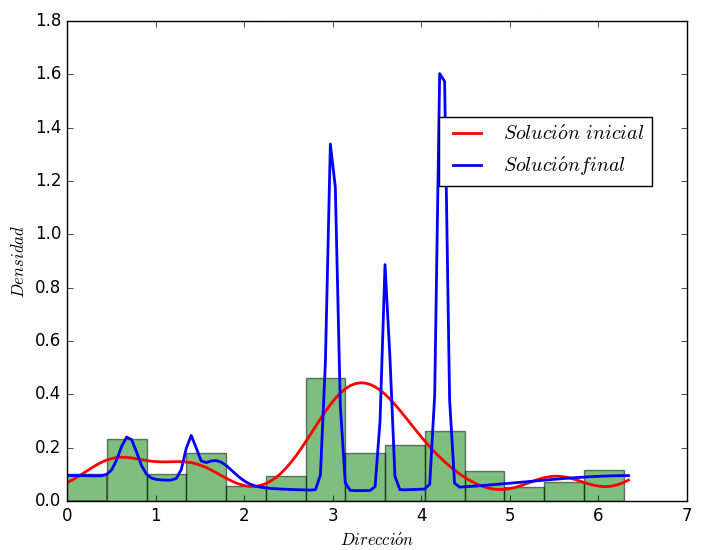
\includegraphics[width=0.45\textwidth]{figures/bad_adjust.png}
        }
        \subfigure[Evolucion de la solución.]{
            \label{fig:EV_SOL}
            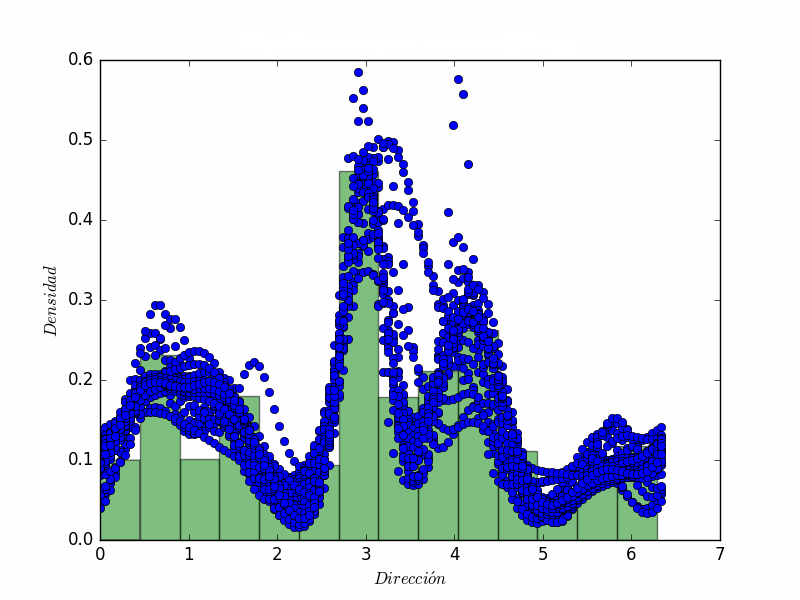
\includegraphics[width=0.45\textwidth]{figures/ev_solution.png}
        }%
    \caption{Pruebas iniciales.}
    \caption*{Fuente: Elaboración propia.}
    \label{fig:subfigures}
\end{figure}

\subsubsection{Experimento 2, Ajustes anuales}
En este experimento se ajustan los vientos anualmente, en los años de los cuales se obtuvieron datos para este estudio, resultado la Figura \ref{fig:SOL_13} para el 2013, la Figura \ref{fig:SOL_14} para el 2014 y la Figura \ref{fig:SOL_15} para el 2015.
Tal como se realiza en otros estudios \cite{Heckenbergerova15} \cite{Winddirelse15}, el ajuste de los datos de dirección del viento en un formato
de largo plazo, permite observar el comportamiento global de los vientos pudiendo evaluar la norma o generalidad en los datos registrados.
En las Figuras referenciadas previamente se observa la evolución de la solución desde la aproximación inicial hasta la mejorada por el PSO.

\begin{figure}[ht!]
     \centering
     \captionsetup{justification=centering,margin=2cm}
        \subfigure[Solución inicial y final, 2015.]{
           \label{fig:SOL_15}
           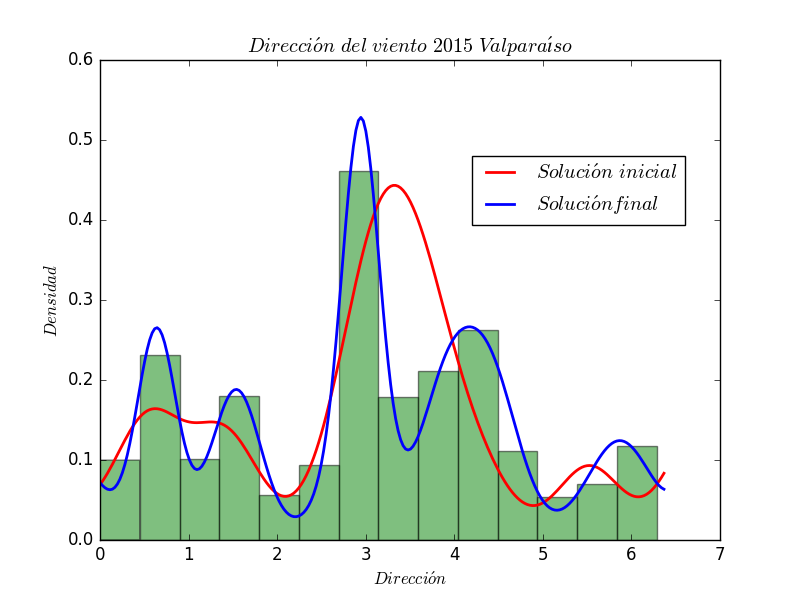
\includegraphics[width=0.45\textwidth]{figures/sol_ini_sol_fin.png}
        }
        \subfigure[Solución inicial y final, 2014.]{
            \label{fig:SOL_14}
            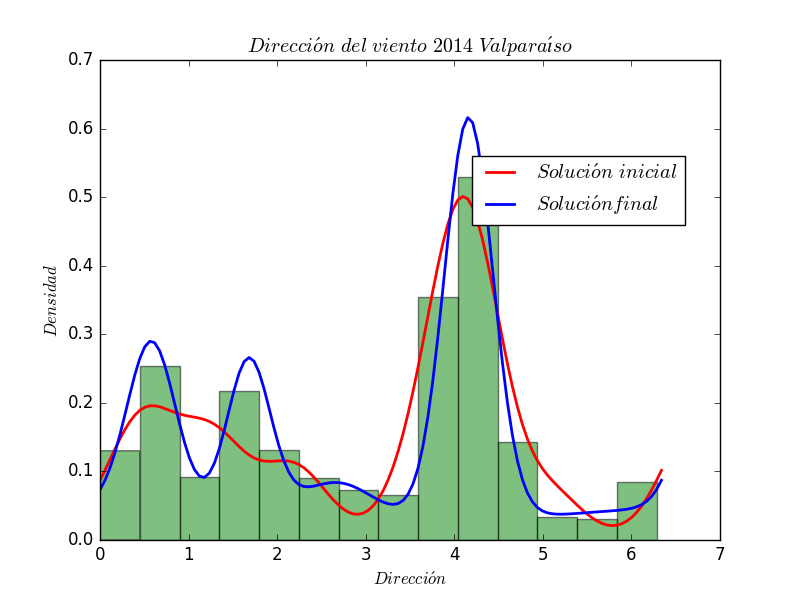
\includegraphics[width=0.45\textwidth]{figures/sol_ini_sol_fin_2014.png}
        }\\
         \subfigure[Solución inicial y final, 2013.]{
            \label{fig:SOL_13}
            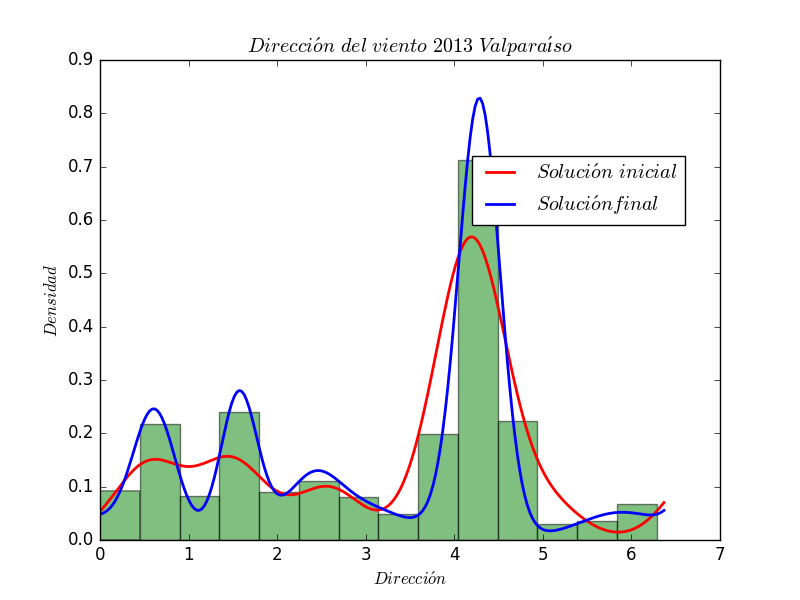
\includegraphics[width=0.45\textwidth]{figures/sol_ini_sol_fin_2013.png}
        }
    \caption{Graficos de ajustes anuales.}
    \caption*{Fuente: Elaboración propia.}
    \label{fig:subfigures}
\end{figure}

\subsubsection{Experimento 3, Ajustes de meses acumulados}
Similar al ejercicio anterior, los gráficos agrupados en \ref{fig:PLOT_MONTHS_ALL_1} y \ref{fig:PLOT_MONTHS_ALL_2}, permiten visualizar el ajuste de los datos del viento por meses. En este caso se agruparon los datos de los tres años escogidos por cada mes, es decir, la Figura \ref{fig:PLOT_SOL_ENERO}, por ejemplo, contiene los datos del mes de enero de los años 2013, 2014 y 2015.\\
Se puede observar que algunos gráficos muestran un mejor ajuste que otros, a pesar del correcto valor obtenido en la función objetivo como se expresa posteriormente en la tabla \ref{table:stadistical_tests_direction}. Esto se debe a que probablemente la solución se escapa más de los deseado de la solución inicial. 
\begin{figure}[ht!]
    \centering
    \captionsetup{justification=centering,margin=2cm}
         %%MONTHS  
        \subfigure[Solución inicial y final, Enero.]{
            \label{fig:PLOT_SOL_ENERO}
            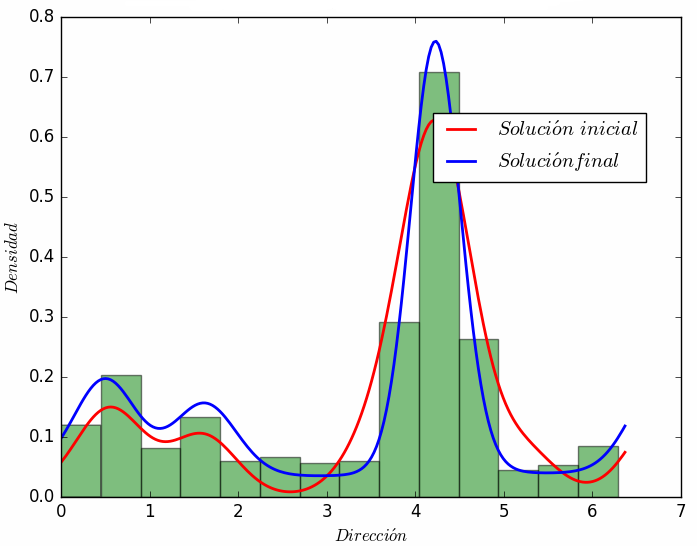
\includegraphics[width=0.42\textwidth]{figures/sol_ini_sol_fin_ENERO.png}
        }
         \subfigure[Solución inicial y final, Febrero.]{
            \label{fig:PLOT_SOL_FEBRERO}
            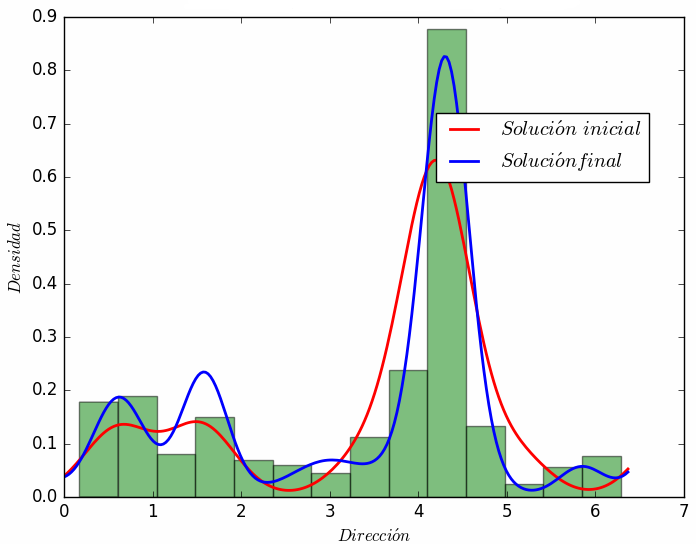
\includegraphics[width=0.42\textwidth]{figures/sol_ini_sol_fin_FEBRERO.png}
        }\\
          \subfigure[Solución inicial y final, Marzo.]{
            \label{fig:PLOT_SOL_MARZO}
            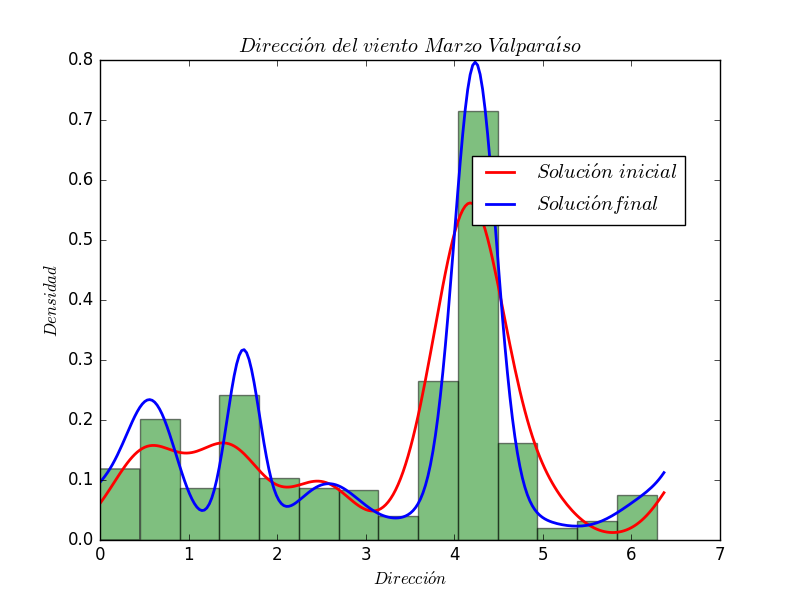
\includegraphics[width=0.42\textwidth]{figures/sol_ini_sol_fin_MARZO.png}
        }
         \subfigure[Solución inicial y final, Abril.]{
            \label{fig:PLOT_SOL_ABRIL}
            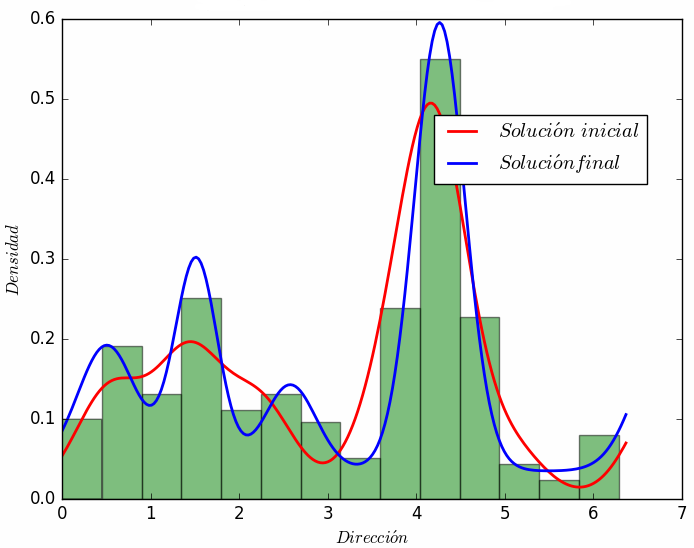
\includegraphics[width=0.42\textwidth]{figures/sol_ini_sol_fin_ABRIL.png}
        }\\
          \subfigure[Solución inicial y final, Mayo.]{
            \label{fig:PLOT_SOL_MAYO}
            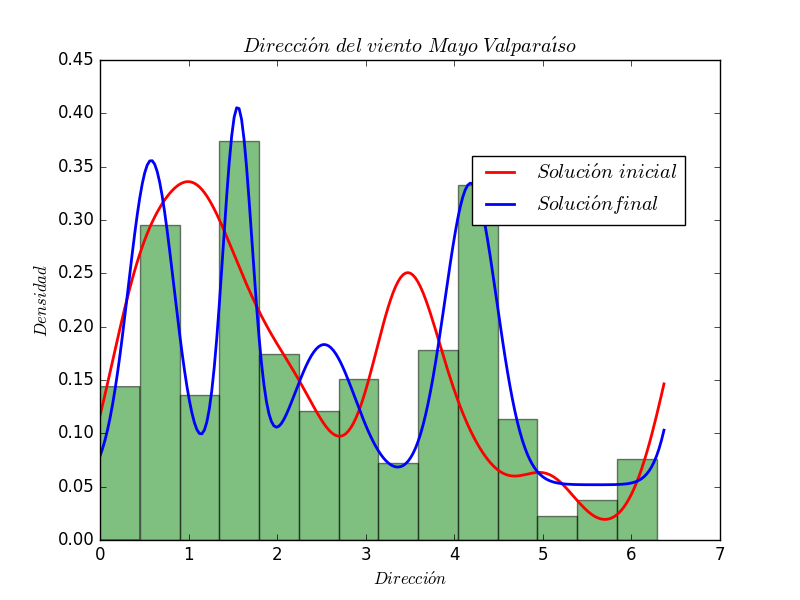
\includegraphics[width=0.42\textwidth]{figures/sol_ini_sol_fin_MAYO.png}
        }
         \subfigure[Solución inicial y final, Junio.]{
            \label{fig:PLOT_SOL_JUNIO}
            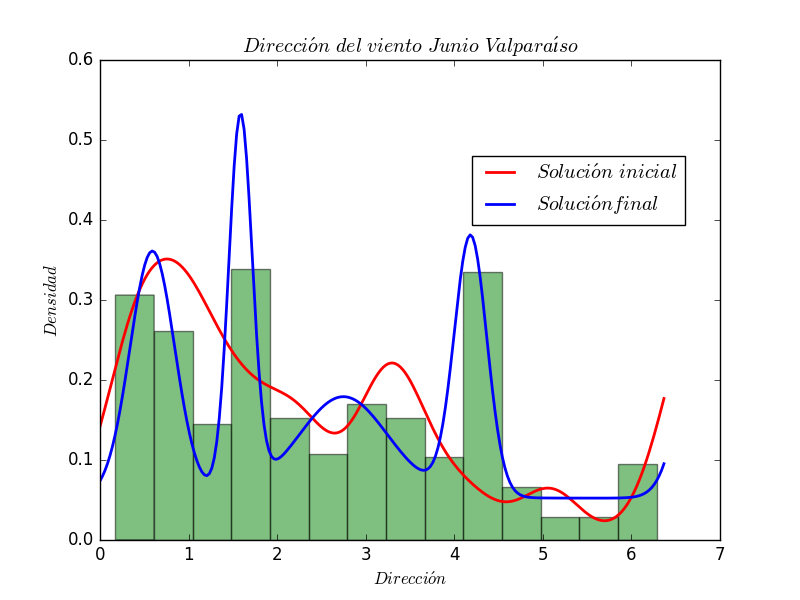
\includegraphics[width=0.42\textwidth]{figures/sol_ini_sol_fin_JUNIO.png}
        }
    \caption{Gráficos de ajuste de MVM por meses.}
    \caption*{Fuente: Elaboración propia.}
    \label{fig:PLOT_MONTHS_ALL_1}
\end{figure}
\newpage
\begin{figure}[ht!]
    \centering
    \captionsetup{justification=centering,margin=2cm}
        \subfigure[Solución inicial y final, Julio.]{
            \label{fig:PLOT_SOL_JULIO}
            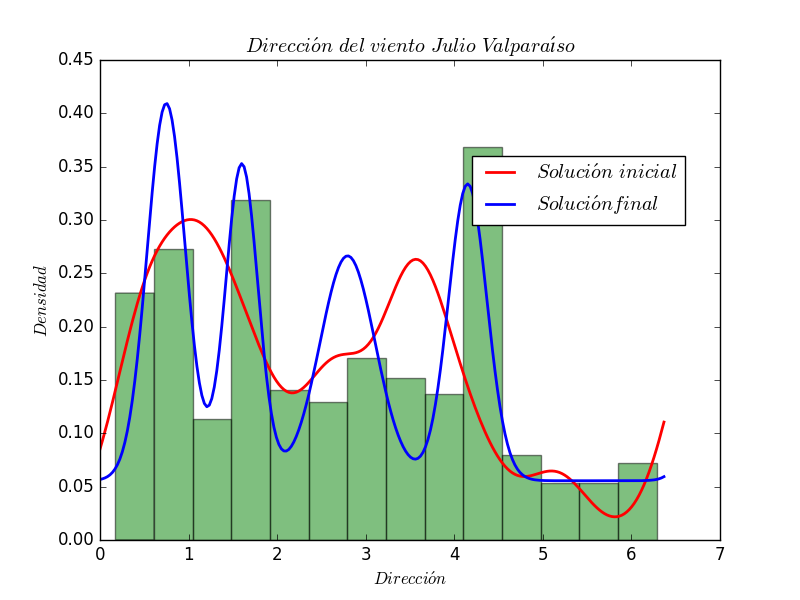
\includegraphics[width=0.42\textwidth]{figures/sol_ini_sol_fin_JULIO.png}
        }
         \subfigure[Solución inicial y final, Agosto.]{
            \label{fig:PLOT_SOL_AGOSTO}
            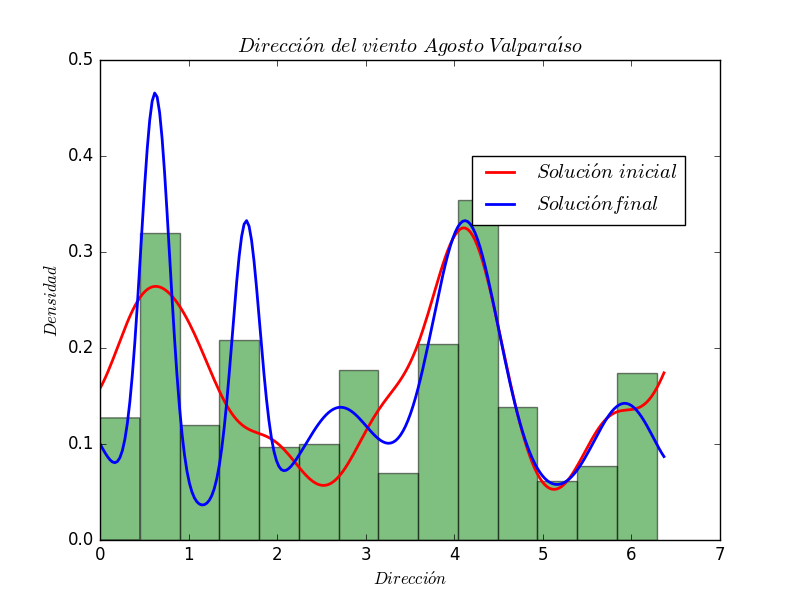
\includegraphics[width=0.42\textwidth]{figures/sol_ini_sol_fin_AGOSTO.png}
        }\\
          \subfigure[Solución inicial y final, Septiembre.]{
            \label{fig:PLOT_SOL_SEPTIEMBRE}
            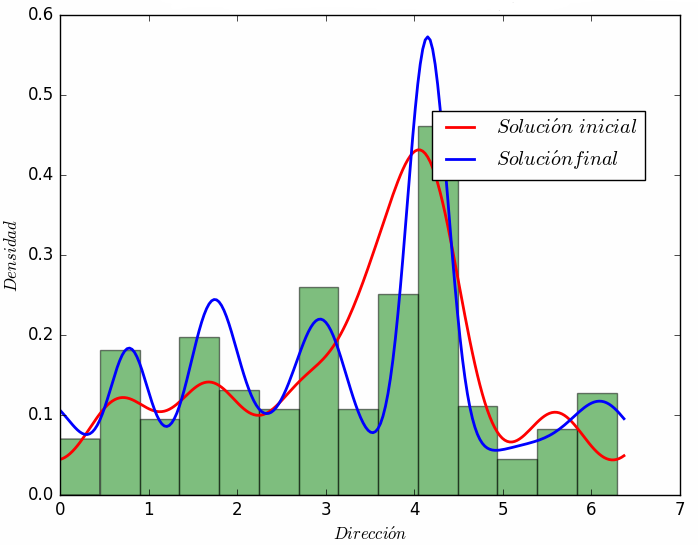
\includegraphics[width=0.42\textwidth]{figures/sol_ini_sol_fin_SEPTIEMBRE.png}
        }
         \subfigure[Solución inicial y final, Octubre.]{
            \label{fig:PLOT_SOL_OCTUBRE}
            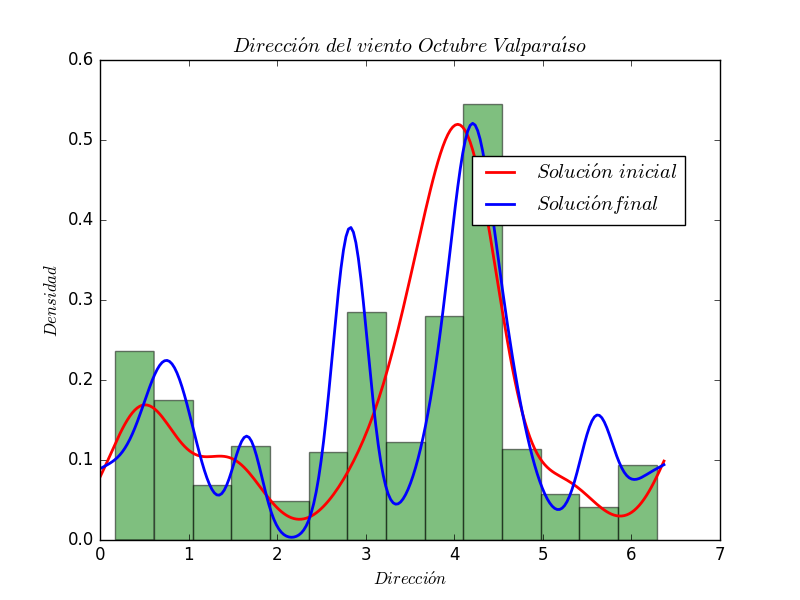
\includegraphics[width=0.42\textwidth]{figures/sol_ini_sol_fin_OCTUBRE.png}
        }\\
          \subfigure[Solución inicial y final, Noviembre.]{
            \label{fig:PLOT_SOL_NOVIEMBRE}
            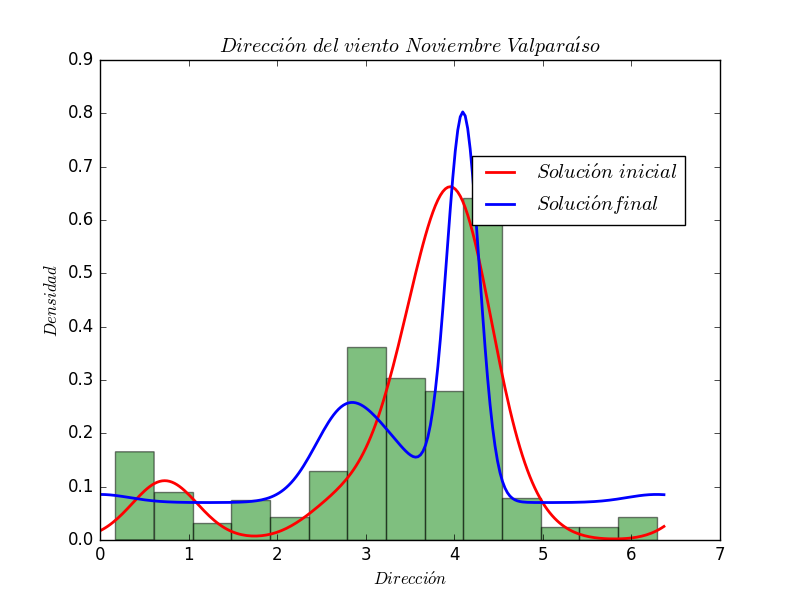
\includegraphics[width=0.42\textwidth]{figures/sol_ini_sol_fin_NOVIEMBRE.png}
        }
         \subfigure[Solución inicial y final, Diciembre.]{
            \label{fig:PLOT_SOL_DICIEMBRE}
            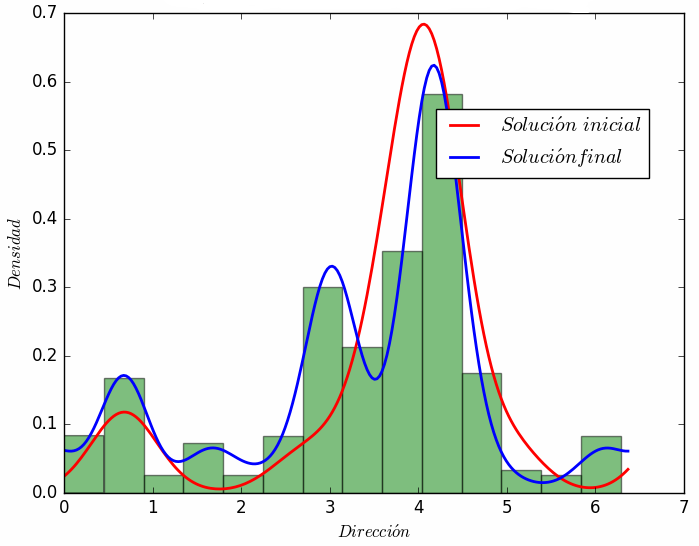
\includegraphics[width=0.42\textwidth]{figures/sol_ini_sol_fin_DICIEMBRE.png}
        }
    \caption{Gráficos de ajuste de MVM por meses.}
    \caption*{Fuente: Elaboración propia.}
    \label{fig:PLOT_MONTHS_ALL_2}
\end{figure}

\subsubsection{Experimento 4, Ajuste por meses, visualización en coordenadas polares}
En las Figuras agrupadas \ref{fig:PLOT_MONTHS_1} y \ref{fig:PLOT_MONTHS_2} se aprecia una visualización más interesante. Allí se puede ver de forma más intuitiva las direcciones dominantes del viento, relativas al sistema de referencia utilizado en meteorología conocido comúnmente como la rosa de los vientos \cite{RosaViento}. En el mes de Enero, Figuras \ref{fig:polar_ene_2015} \ref{fig:polar_ene_2014} \ref{fig:polar_ene_2013}, los vientos parecen provenir principalmente desde el suroeste, mientras que en Mayo, Figuras \ref{fig:polar_may_2015} \ref{fig:polar_may_2014} \ref{fig:polar_may_2013}, el origen del viento es más variable, proviniendo desde el noreste y el sur principalmente. En Septiembre, Figuras \ref{fig:polar_sep_2015} \ref{fig:polar_sep_2014} \ref{fig:polar_sep_2013}, vuelve a ser una fuente de los vientos predominante el suroeste.
\begin{figure}[ht!]
    \centering
    \captionsetup{justification=centering,margin=2cm}
        \subfigure[Dirección enero 2015.]{
            \label{fig:polar_ene_2015}
            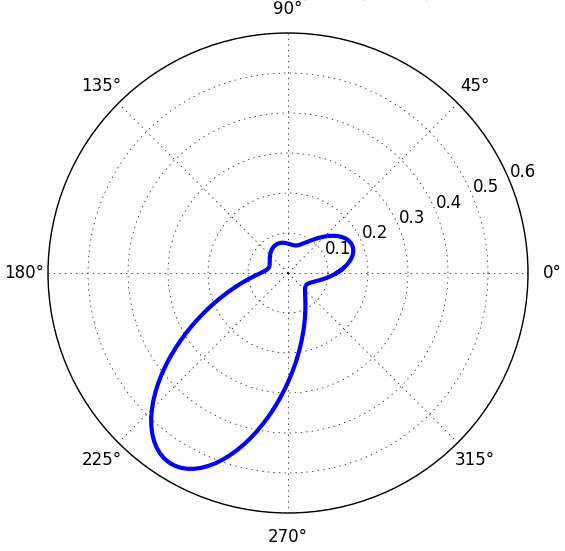
\includegraphics[width=0.43\textwidth]{figures/direction_enero_2015.png}
        }
         \subfigure[Dirección enero 2014.]{
            \label{fig:polar_ene_2014}
            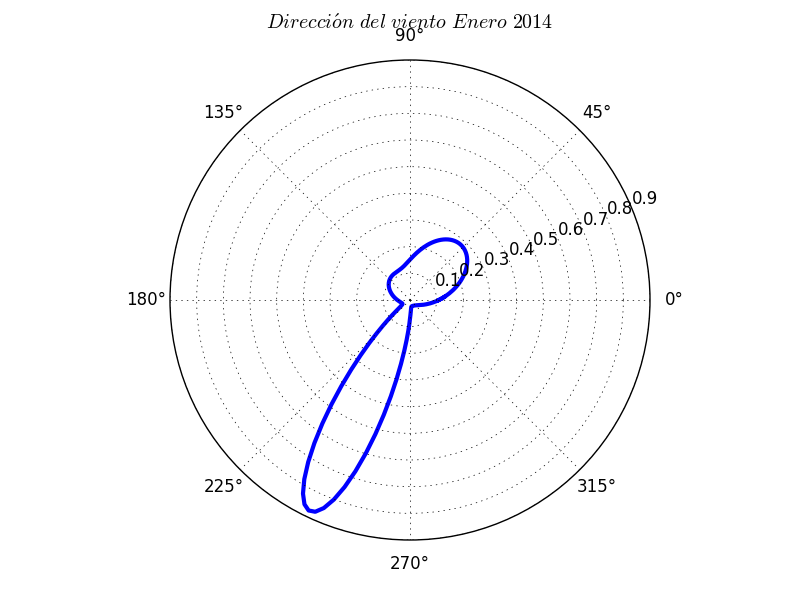
\includegraphics[width=0.43\textwidth]{figures/direction_enero_2014.png}
        }\\
         \subfigure[Dirección enero 2013.]{
            \label{fig:polar_ene_2013}
            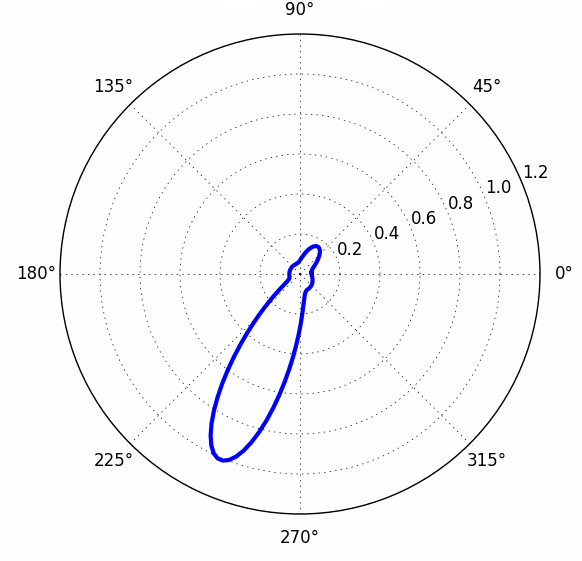
\includegraphics[width=0.43\textwidth]{figures/direction_enero_2013.png}
        }
         \subfigure[Dirección mayo 2015.]{
            \label{fig:polar_may_2015}
            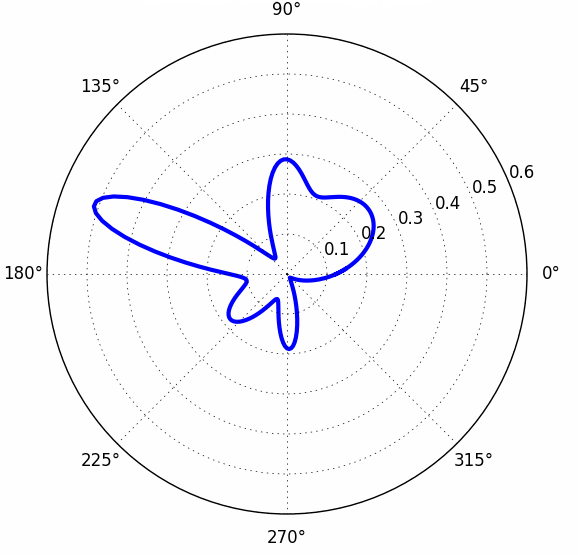
\includegraphics[width=0.43\textwidth]{figures/direction_mayo_2015.png}
        }\\
         \subfigure[Dirección mayo 2014.]{
            \label{fig:polar_may_2014}
            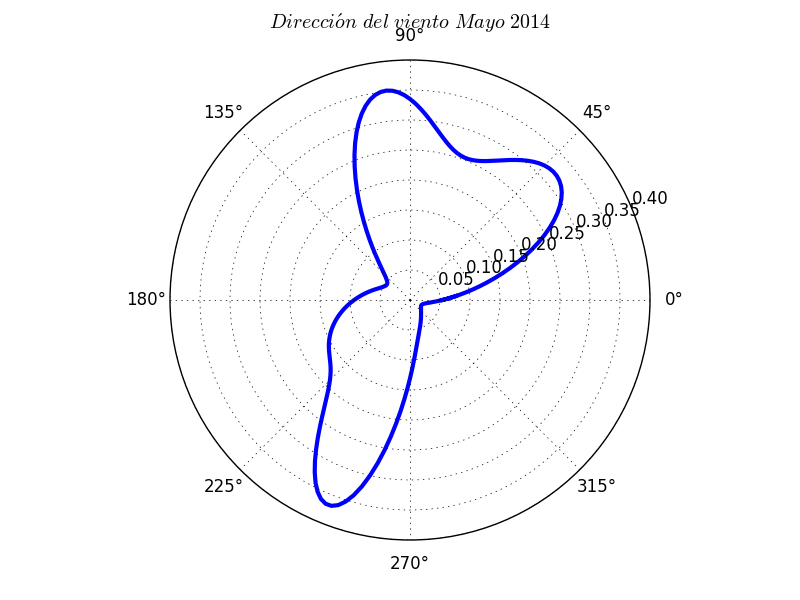
\includegraphics[width=0.43\textwidth]{figures/direction_mayo_2014.png}
        }
         \subfigure[Dirección mayo 2013.]{
            \label{fig:polar_may_2013}
            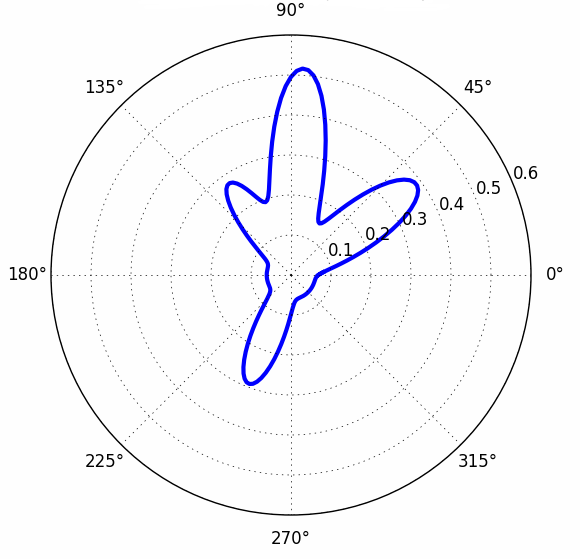
\includegraphics[width=0.43\textwidth]{figures/direction_mayo_2013.png}
        }
    \caption{Gráficos de ajuste por meses en coordenadas polares.}
    \caption*{Fuente: Elaboración propia.}
    \label{fig:PLOT_MONTHS_1}
\end{figure}

\begin{figure}[ht!]
    \centering
    \captionsetup{justification=centering,margin=2cm}
        \subfigure[Dirección septiembre 2015.]{
            \label{fig:polar_sep_2015}
            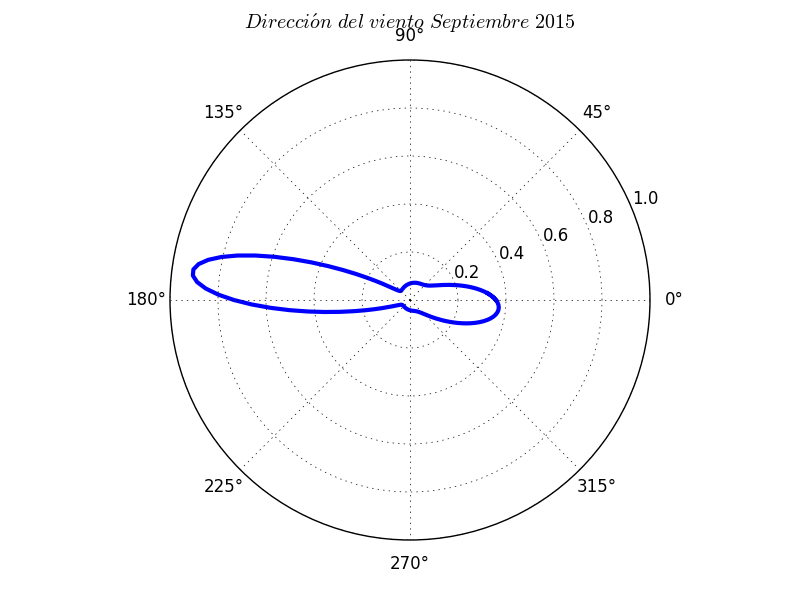
\includegraphics[width=0.45\textwidth]{figures/direction_septiembre_2015.png}
        }
         \subfigure[Dirección septiembre 2014.]{
            \label{fig:polar_sep_2014}
            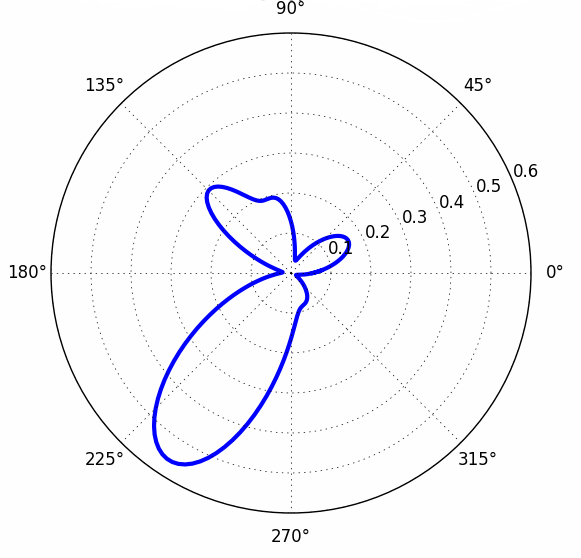
\includegraphics[width=0.45\textwidth]{figures/direction_septiembre_2014.png}
        }\\
         \subfigure[Dirección septiembre 2013.]{
            \label{fig:polar_sep_2013}
            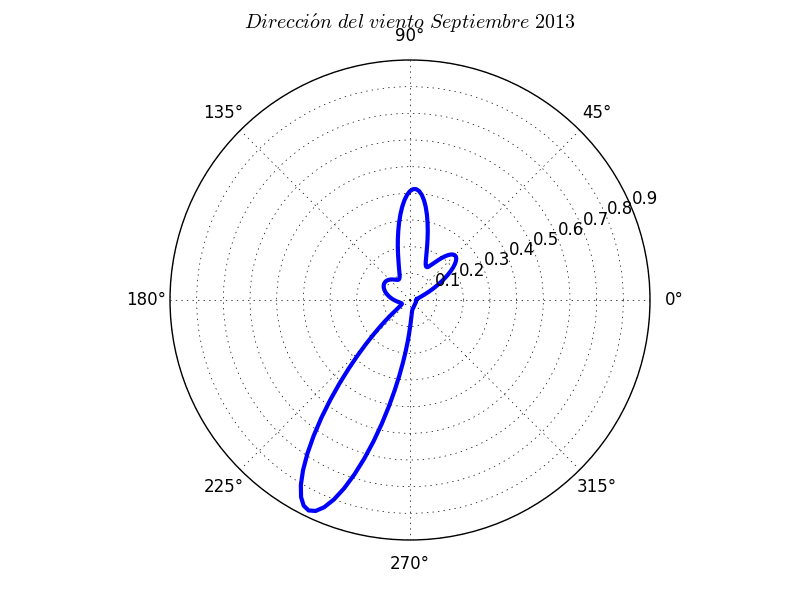
\includegraphics[width=0.45\textwidth]{figures/direction_septiembre_2013.png}
        }  
    \caption{Gráficos de ajuste por meses en coordenadas polares.}
    \caption*{Fuente: Elaboración propia.}
    \label{fig:PLOT_MONTHS_2}
\end{figure}

\subsubsection{Resumen de los experimentos}
%\begin{table}[ht!]
%    %\centering
%    \caption{Tabla de pruebas, PSO dirección del viento}
%    \label{table:stadistical_tests_direction}
%    \resizebox{\textwidth}{!}{
%    \begin{tabular}{|c|c|c|c|c|c|c|c|c|}
%        \hline
%        \textbf{Periodo de tiempo} & \textbf{PSI} & \textbf{PSFV} & \textbf{PSFF} & \textbf{Tiempo V} & \textbf{Tiempo F} & \textbf{Iteraciones V} & \textbf{%Iteraciones F} & \textbf{Cantidad datos}\\
%        \hline
%        2015            & 461,83    & -         & 251,37    & -           & 38m46,1s    & -     & 50500 & 2076 \\
%        2015            & 461,83    & 21,58     & 234,97    & 8m5,7s      & 47m47,1s    & 9005  & 50500 & 2076 \\
%        2014            & 301,12    & 24,86     & 56,57     & 20m37,8s    & 46m23,2s    & 29494 & 50500 & 2499 \\ 
%        2013            & 424,24    & 33,76     & 69,53     & 11m41,1s    & 48m23,7s    & 16778 & 50500 & 2346 \\
%        \hline
%        Enero           & 144,42    & 20,89     & 22,18     & 0m3,3s      & 25m37,2s    & 86    & 27276 & 633 \\
%        Febrero         & 130,39    & 19,45     & 22,27     & 0m12,2s     & 0m07,1s     & 288   & 134   & 567\\
%        Marzo           & 104,54    & 18,61     & 22,31     & 0m3,1s      & 0m13,3s     & 49    & 228   & 564 \\
%        Abril           & 74,97     & 21,13     & 22,25     & 0m12,5s     & 17m58,4s    & 192   & 18544 & 559 \\
%        Mayo            & 243,65    & 21,65     & 81,75     & 1m6,9s      & 42m59,6s    & 1237  & 50000 & 589 \\
%        Junio           & 286,30    & 21,01     & 188,91    & 1m42,9s     & 40m52,5s    & 1989  & 50000 & 554 \\
%        Julio           & 177,33    & 22,06     & 31,39     & 0m17,8s     & 45m48,3s    & 315   & 50000 & 604 \\
%        Agosto          & 79,57     & 21,94     & 22,17     & 0m12,9s     & 40m26,3s    & 202   & 41204 & 578 \\
%        Septiembre      & 92,77     & 21,31     & 22,31     & 0m1,7s      & 0m1,7s      & 27    & 166   & 541 \\
%        Octubre         & 188,14    & 21,81     & 37,50     & 0m45,3s     & 42m56,4s    & 825   & 50000 & 564 \\
%        Noviembre       & 363,90    & 26,25     & 88,16     & 42m21,4s    & 42m53,6s    & 50500 & 50000 & 582 \\
%        Diciembre       & 335,28    & 22,30     & 37,81     & 9m56,1s     & 43m52,9s    & 11640 & 50000 & 586 \\
%        \hline 
%        Enero 2015      & 42,94     & 16,34     & 18,77     & 0m4,1s      & 0m0,1s      & 61    & 10    & 220 \\
%        Enero 2014      & 68,10     & 20,68     & 21,61     & 0m1,8s      & 0m0,7s      & 29    & 126   & 206 \\
%        Enero 2013      & 194,98    & 19,31     & 24,86     & 0m0,4s      & 46m29,2s    & 6     & 50000 & 207 \\
%        Mayo 2015       & 60,84     & 17,99     & 26,69     & 0m2,3s      & 41m53,8s    & 39    & 50000 & 173 \\
%        Mayo 2014       & 142,85    & 20,94     & 20,48     & 0m4,8s      & 0m0,3s      & 82    & 50    & 213 \\
%        Mayo 2013       & 135,68    & 20,88     & 22,34     & 0m5,3s      & 0m1,1s      & 97    & 2089  & 203 \\
%        Septiembre 2015 & 77,41     & 21,29     & 25,54     & 0m8,4s      & 41m48,7s    & 137   & 50000 & 140 \\
%        Septiembre 2014 & 19,56     & 18,24     & 15,86     & 0m0,1s      & 0m0,1s      & 1     & 1     & 200 \\
%        Septiembre 2013 & 68,90     & 16,61     & 21,89     & 0m0,3s      & 0m0,9s      & 5     & 150   & 201 \\
%        \hline  
%    \end{tabular}
%    }   
%\end{table}

\begin{table}[ht!]
    %\centering
    \caption{Tabla de pruebas y repeticiones, PSO dirección del viento, Estrategia Variable}
    \label{table:repetitions_tests_direction_variable}
    \resizebox{\textwidth}{!}{
    \begin{tabular}{|c|c|c|c|c|c|c|c|c|c|c|c|}
        \hline
        \textbf{Periodo de tiempo} & \textbf{Puntaje Inicial} & \textbf{Menor Puntaje} & \textbf{Mayor Puntaje} & \textbf{Promedio Puntaje} & \textbf{Menor Iteraciones} & \textbf{Mayor Iteraciones} & \textbf{Promedio Iteraciones} & \textbf{Menor Tiempo} & \textbf{Mayor Tiempo} & \textbf{Promedio Tiempo} & \textbf{Cantidad datos}\\
        \hline
        2015            & 461,83    & 19,42     & 86,60  & 32,11 & 445   & 26395 & 13314 & 34   & 1800  &  992   & 2076 \\
        2014            & 301,12    & 17,08     & 59,73  & 36,18 & 4914  & 25904 & 22633 & 359  & 1800  &  1655  & 2499 \\ 
        2013            & 424,24    & 17,94     & 81,44  & 26,24 & 838   & 26048 & 12307 & 65   & 1800  &  925   & 2346 \\
        \hline  
        Enero           & 144,42    & 20,75     & 22,33  & 21,76 & 22    & 22515 & 1918  & 1    & 1558  & 136    & 633 \\
        Febrero         & 130,39    & 17,69     & 24,24  & 21,70 & 185   & 27321 & 3978  & 14   & 1800  & 277    & 567\\
        Marzo           & 104,54    & 16,90     & 24,38  & 21,57 & 37    & 25994 & 2448  & 3    & 1800  & 174    & 564 \\
        Abril           & 74,97     & 17,19     & 22,35  & 21,20 & 41    & 3369  & 589   & 3    & 235   & 42     & 559 \\
        Mayo            & 243,65    & 18,86     & 22,34  & 21,46 & 58    & 2281  & 559   & 4    & 166   & 41     & 589 \\
        Junio           & 286,30    & 20,36     & 22,35  & 21,98 & 50    & 2229  & 754   & 4    & 161   & 55     & 554 \\
        Julio           & 177,33    & 16,29     & 22,33  & 21,12 & 53    & 585   & 258   & 4    & 43    & 19     & 604 \\
        Agosto          & 79,57     & 16,42     & 22,30  & 20,99 & 12    & 2155  & 208   & 1    & 171   & 16     & 578 \\
        Septiembre      & 92,77     & 14,48     & 22,34  & 20,55 & 16    & 227   & 70    & 1    & 18    & 6      & 541 \\
        Octubre         & 188,14    & 19,21     & 24,41  & 21,89 & 300   & 25702 & 6607  & 22   & 1800  & 479    & 564 \\
        Noviembre       & 363,90    & 21,90     & 46,00  & 27,00 & 2288  & 25956 & 23969 & 168  & 1800  & 1725   & 582 \\
        Diciembre       & 335,28    & 21,55     & 64,28  & 27,68 & 5179  & 28004 & 20210 & 364  & 1800  & 1364   & 586 \\
        \hline 
        Enero 2015      & 42,94     & 18,68     & 22,33  & 20,50 & 3     & 81    & 29    & 1    & 6     &  2     & 220 \\
        Enero 2014      & 68,10     & 16,71     & 22,35  & 20,39 & 7     & 438   & 61    & 1    & 32    &  5     & 206 \\
        Enero 2013      & 194,98    & 15,41     & 22,30  & 19,98 & 10    & 245   & 76    & 1    & 19    &  6     & 207 \\
        Mayo 2015       & 60,84     & 17,68     & 22,28  & 20,97 & 5     & 107   & 38    & 1    & 8     &  3     & 173 \\
        Mayo 2014       & 142,85    & 16,30     & 22,30  & 20,22 & 9     & 52    & 24    & 1    & 4     &  2     & 213 \\
        Mayo 2013       & 135,68    & 15,16     & 21,99  & 19,86 & 2     & 159   & 24    & 1    & 13    &  2     & 203 \\
        Septiembre 2015 & 77,41     & 11,13     & 22,29  & 19,70 & 8     & 2529  & 690   & 1    & 219   &  60    & 140 \\
        Septiembre 2014 & 19,56     & 11,01     & 22,31  & 19,54 & 1     & 27    & 10    & 1    & 2     &  1     & 200 \\
        Septiembre 2013 & 68,90     & 12,29     & 22,33  & 19,92 & 10    & 175   & 35    & 1    & 12    &  3     & 201 \\
        \hline  
    \end{tabular}
    }   
\end{table}

\begin{table}[ht!]
    %\centering
    \caption{Tabla de pruebas y repeticiones, PSO dirección del viento, Estrategia Fija}
    \label{table:repetitions_tests_direction_fijo}
    \resizebox{\textwidth}{!}{
    \begin{tabular}{|c|c|c|c|c|c|c|c|c|c|c|c|}
        \hline
        \textbf{Periodo de tiempo} & \textbf{Puntaje Inicial} & \textbf{Menor Puntaje} & \textbf{Mayor Puntaje} & \textbf{Promedio Puntaje} & \textbf{Menor Iteraciones} & \textbf{Mayor Iteraciones} & \textbf{Promedio Iteraciones} & \textbf{Menor Tiempo} & \textbf{Mayor Tiempo} & \textbf{Promedio Tiempo} & \textbf{Cantidad datos}\\
        \hline
        2015            & 461,83    & 51,79     & 380,40  & 137,07 & 24082  & 27506 & 25651 & 1800 & 1800  & 1800  & 2076 \\
        2014            & 301,12    & 62,07     & 314,62  & 122,52 & 21681  & 26393 & 24633 & 1800 & 1800  & 1800  & 2499 \\
        2013            & 424,24    & 65,76     & 433,80  & 182,85 & 21684  & 27603 & 23866 & 1800 & 1800  & 1800  & 2346 \\
        \hline  
        Enero           & 144,42    & 22,30     & 96,99   & 49,17 & 940     & 26675 & 23210 & 68   & 1800  & 1699  & 633 \\
        Febrero         & 130,39    & 23,20     & 87,79   & 46,30 & 22926   & 26619 & 24898 & 1800 & 1800  & 1800  & 567\\
        Marzo           & 104,54    & 21,15     & 106,97  & 45,49 & 376     & 26552 & 22377 & 28   & 1800  & 1647  & 564 \\
        Abril           & 74,97     & 19,82     & 84,00   & 33,61 & 54      & 27723 & 13408 & 5    & 1800  & 948   & 559 \\
        Mayo            & 243,65    & 21,98     & 52,87   & 28,44 & 212     & 25973 & 20789 & 16   & 1800  & 1519  & 589 \\
        Junio           & 286,30    & 22,76     & 188,91  & 50,13 & 20320   & 27830 & 23479 & 1668 & 1800  & 1756  & 554 \\
        Julio           & 177,33    & 23,05     & 72,56   & 33,93 & 127     & 26587 & 21869 & 55   & 1800  & 1533  & 604 \\
        Agosto          & 79,57     & 20,45     & 78,96   & 25,72 & 66      & 25514 & 19256 & 7    & 1800  & 1623  & 578 \\
        Septiembre      & 92,77     & 21,30     & 64,74   & 32,17 & 155     & 27258 & 20122 & 47   & 1800  & 1414  & 541 \\
        Octubre         & 188,14    & 22,35     & 102,38  & 38,70 & 277     & 26231 & 24109 & 36   & 1800  & 1563  & 564 \\
        Noviembre       & 363,90    & 32,69     & 150,89  & 63,91 & 359     & 26032 & 22324 & 20   & 1800  & 1899  & 582 \\
        Diciembre       & 335,28    & 24,35     & 90,86   & 47,12 & 15720   & 27111 & 21662 & 89   & 1800  & 1657  & 586 \\
        \hline 
        Enero 2015      & 42,94     & 15,24     & 38,07   & 22,51 & 17      & 27010  & 8265  & 1   & 1800   & 586  & 220 \\
        Enero 2014      & 68,10     & 17,16     & 32,71   & 21,78 & 11      & 26014  & 7265  & 1   & 1800   & 750  & 206 \\
        Enero 2013      & 194,98    & 14,58     & 41,95   & 30,89 & 6       & 25341  & 6541  & 1   & 1800   & 789  & 207 \\
        Mayo 2015       & 60,84     & 16,92     & 35,77   & 25,72 & 21      & 20147  & 7566  & 1   & 1800   & 852  & 173 \\
        Mayo 2014       & 142,85    & 19,32     & 56,89   & 30,88 & 62      & 24612  & 7894  & 3   & 1800   & 421  & 213 \\
        Mayo 2013       & 135,68    & 18,26     & 46,33   & 33,90 & 44      & 20144  & 8742  & 1   & 1800   & 520  & 203 \\
        Septiembre 2015 & 77,41     & 19,52     & 30,45   & 21,14 & 79      & 24700  & 8440  & 2   & 1800   & 324  & 140 \\
        Septiembre 2014 & 19,56     & 14,36     & 29,51   & 24,55 & 1       & 20892  & 3247  & 1   & 1800   & 385  & 200 \\
        Septiembre 2013 & 68,90     & 16,86     & 32,48   & 22,63 & 5       & 24113  & 4570  & 1   & 1800   & 480  & 201 \\
        \hline  
    \end{tabular}
    }   
\end{table}

\begin{figure}[ht!]
    \centering
    \captionsetup{justification=centering,margin=2cm}
        \subfigure[Puntajes obtenidos con la estrategia Variable.]{
            \label{fig:polar_ene_2015}
            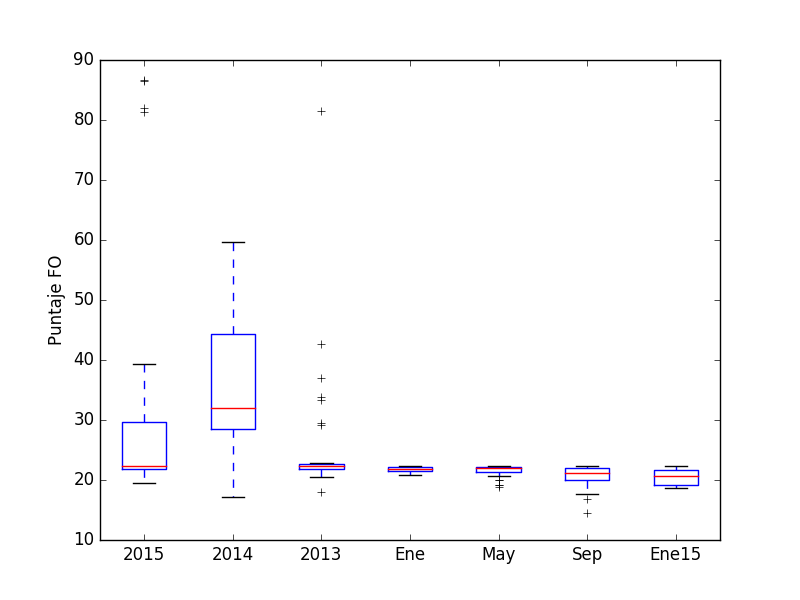
\includegraphics[width=0.45\textwidth]{figures/bp_puntaje_V.png}
        }
         \subfigure[Puntajes obtenidos con la estrategia Fija.]{
            \label{fig:polar_ene_2014}
            \includegraphics[width=0.45\textwidth]{figures/bp_puntaje_F.png}
        }\\
         \subfigure[Iteraciones alcanzadas con la estrategia Variable.]{
            \label{fig:polar_ene_2013}
            \includegraphics[width=0.45\textwidth]{figures/bp_iteraciones_V.png}
        }
         \subfigure[Iteraciones alcanzadas con la estrategia Fija.]{
            \label{fig:polar_may_2015}
            \includegraphics[width=0.45\textwidth]{figures/bp_iteraciones_F.png}
        }\\
         \subfigure[Tiempos empleado con la estrategia Variable.]{
            \label{fig:polar_may_2014}
            \includegraphics[width=0.45\textwidth]{figures/bp_tiempo_V.png}
        }
         \subfigure[Tiempos empleado con la estrategia Fija.]{
            \label{fig:polar_may_2013}
            \includegraphics[width=0.45\textwidth]{figures/bp_tiempo_F.png}
        }
    \caption{Boxplots de repeticiones del PSO con al estratégia Fija y Variable.}
    \caption*{Fuente: Elaboración propia.}
    \label{fig:BOXPLOTS_DIRECTION}
\end{figure}


Las tablas \ref{table:repetitions_tests_direction_variable} y \ref{table:repetitions_tests_direction_fijo} muestran un resumen de los resultados obtenidos al ajustar la distribución de probabilidad \emph{von Mises distribution} en diferentes subconjuntos de tiempo de los datos colectados en los años 2013, 2014 y 2015, siguiendo la estrategia Variable (propuesta en esta memoria) y la estrategia Fija (sin variación de parámetros). Las tablas están organizadas como sigue a continuación. La estrategia \textbf{Variable} hace referencia a la propuesta realizada en esta memoria para la variación de parámetros del PSO explicada en la sección \ref{subsec:parametros_new}, mientras que la estrategia \textbf{Fijo} es la seguida en el trabajo de Heckenbergerova et al. \cite{Heckenbergerova15}, la cual consta de la definición de parámetros fijos para el PSO.
\begin{enumerate}
    \item \emph{Periodo de tiempo}: Rango de tiempo donde se consideraron los datos para el ajuste.
    \item \emph{Puntaje Inicial}: Puntaje solución inicial, es decir, el valor obtenido al evaluar la solución inicial en la función objetivo.
    \item \emph{Menor Puntaje}: Equivale al mejor puntaje obtenido por las repeticiones.
    \item \emph{Mayor Puntaje}: Equivale al peor puntaje obtenido por las repeticiones.
    \item \emph{Promedio Puntaje}: Puntaje promedio de las repeticiones.
    \item \emph{Menor Iteraciones}: Equivale a la mejor cantidad de iteraciones obtenidas por las repeticiones.
    \item \emph{Mayor Iteraciones}: Equivale a la mejor cantidad de iteraciones obtenidas por las repeticiones. 
    \item \emph{Promedio Iteraciones}: Iteraciones promedio de las repeticiones. 
    \item \emph{Menor Tiempo}: Equivale al mejor tiempo obtenido por las repeticiones.
    \item \emph{Mayor Tiempo}: Equivale al peor tiempo obtenido por las repeticiones.
    \item \emph{Promedio Tiempo}: Tiempo promedio de las repeticiones.
    \item \emph{Cantidad datos}: Cantidad de datos utilizados en el ajuste.
\end{enumerate}

\begin{figure}[ht!]
    \centering
    \captionsetup{justification=centering,margin=2cm}
        \includegraphics[width=\textwidth]{figures/comp_v1_v2_iteraciones.png}
        \includegraphics[width=\textwidth]{figures/comp_v1_v2_puntaje.png} 
    \caption{Comparación de variaciones en el PSO.}
    \caption*{Fuente: Elaboración propia.}
    \label{fig:comparison_pso_1}
\end{figure}

\begin{figure}[ht!]
    \centering
    \captionsetup{justification=centering,margin=2cm}
        \includegraphics[width=\textwidth]{figures/comp_v1_v2_tiempo.png}   
    \caption{Comparación de variaciones en el PSO.}
    \caption*{Fuente: Elaboración propia.}
    \label{fig:comparison_pso_2}
\end{figure}
Los gráficos en \ref{fig:comparison_pso_1} y  \ref{fig:comparison_pso_2} muestran la comparación de los rendimientos de los algoritmos con parámetros fijos y variables para el PSO según la propuesta explicada en la sección \ref{subsec:parametros_new}. Es claro que en la mayoría de los experimentos, la propuesta realizada tiene mejor rendimiento y en el peor de los casos se comporta igual o levemente peor que la forma tradicional de parámetros fijos utilizada en el trabajo de Heckenbergerova et al. \cite{Heckenbergerova15}.\\
En las Figuras en \ref{fig:BOXPLOTS_DIRECTION}, se pueden observar la distribución de resultados para los puntajes, iteraciones y tiempos obtenidos por las repeticiones de algunos de los experimentos. En general los valores alcanzados son similares independiente de la semilla generadora de números aleatorios, a excepción de algunos casos particulares en donde se observa una alta dispersión, sobre todo en los experimentos del PSO con estrategia Fija.
\newpage
\section{Conclusiones del capítulo}
En este capítulo se ajustaron los parámetros de la función \emph{mixture of von Mises distribution} a datos de dirección del viento en Valparaíso. Basado en el trabajo de Heckenbergerova et al. \cite{Heckenbergerova15}, se implementó el \emph{Particle Swarm Optimization} con una modificación propuesta en esta memoria para mejorar los resultados del trabajo citado.\\
Como se puede ver en la tabla \ref{table:stadistical_tests_direction}, la modificación propuesta y explicada en las ecuaciones \ref{eq:VariationParameters_new}, \ref{eq:VariationParameters_new_2} y \ref{eq:VariationParameters_new_3} para el control de los parámetros del PSO, permite obtener mejores tiempos de ejecución y soluciones de mejor calidad que los valores utilizados en el trabajo de Heckenbergerova et al. \cite{Heckenbergerova15}. Esto se debe al problema de convergencia prematura del PSO, el cual no fue considerado en dicho trabajo. \\
De las Figuras expuestas en \ref{fig:PLOT_MONTHS_ALL_1} y \ref{fig:PLOT_MONTHS_ALL_2} se puede observar que a pesar del buen puntaje conseguido por la solución, el gráfico difiere del histograma en varias pruebas más de lo deseado. Esto se debe a que la función objetivo definida en el PSO procura que las áreas bajo la curva de la función de densidad de probabilidad coincidan con las del histograma, sin embargo, más de una forma de la función de densidad puede cumplir dicho objetivo. Para evitar este problema se podría modificar la función objetivo añadiendo una penalización a la distancia de los puntos de la curva con respecto a la altura de la sección del histograma correspondiente.\\
Finalmente, al variar la semilla de números aleatorios, se observa una mayor dispersión en los resultados obtenidos del PSO con la estrategia Fija (sin variar los parámetros del algoritmo durante la ejecución) en comparación con la propuesta realizada en esta memoria.
%!TEX root = main.tex

\chapter{Aplicaciones}
En esta sección se explicará a modo general el uso de la técnica propuesta y las potenciales aplicaciones que tienen los resultados obtenidos.
\section{Esquema de uso del algoritmo}
El esquema \ref{esq:PSO_ALG} resume el funcionamiento del algoritmo para el ajuste del modelo probabilístico a los datos del viento. A continuación se detallarán los pasos a seguir en el proceso de obtener el ajuste de parámetros de la distribución elegida.
\begin{enumerate}
    \item Lo primero que se realiza es el formateo de los datos, es decir, la conversión desde un conjunto de mediciones al formato utilizado por el programa desarrollado, en este caso se utiliza el \emph{comma-separated values} CSV. El \emph{script} utilizado dependerá del formato externo del cual provengan los datos.
    \item Una vez obtenidos los datos en el formato deseado, se procede a calcular las frecuencias de los registros obtenidos, para posteriormente ser comparadas con el modelo teórico. El número de frecuencias está determinado por la cantidad de subgrupos definidos que representan intervalos de datos.
    \item Antes de comenzar con el ajuste, se calcula una solución inicial ya sea de forma aleatoria (como es el caso para el ajuste de la velocidad del viento) o mediante algún método conveniente (como la aproximación numérica para el caso del ajuste de la dirección del viento).  
    \item Definiendo la cantidad de partículas y el número de iteraciones, se ejecuta el algoritmo \emph{Particle Swarm Optimization} para que mejore la estimación inicial de acuerdo a una función objetivo previamente definida. 
    \item Finalmente, una vez que el algoritmo termina, entrega los valores de los parámetros para la función de densidad de probabilidad (fdp) elegida. En esta memoria se utilizaron la distribución de Weibull y la \emph{mixture of von Mises distribution}. Con ello, es posible elaborar un histograma y graficar la fdp para evaluar el ajuste obtenido.
\end{enumerate}
En meteorología, la velocidad del viento se registra en nudos por segundo, pero en esta memoria se convirtieron los datos de acuerdo al sistema internacional SI, o sea, a metros por segundo. La conversión consta en multiplicar el valor de los nudos/segundo por 0.514444 para obtener los metros/segundo correspondientes, como se describe en el libro de unidades internacionales de medidas de la Universidad de Illinois \cite{KnotsMeterSeconds}.\\
El sistema de referencia utilizado para la interpretación de los datos de dirección del viento es el conocido como la rosa de los vientos \cite{RosaViento}. Dicho sistema ubica el Norte en el grado 0, al Este en el grado 90, al Sur en el grado 180 y al Oeste en el grado 270, siendo la dirección determinada el origen desde donde proviene el viento. Ejemplo, si la dirección predominante del viento en cierto intervalo de tiempo es de 90 grados, entonces diremos que la corriente de viento proviene desde el este.

\begin{figure}[ht!]
\caption{Esquema de uso del algoritmo}
% Define block styles
\tikzstyle{decision} = [diamond, draw, fill=blue!20, 
    text width=4.5em, text badly centered, node distance=3cm, inner sep=0pt]
\tikzstyle{block} = [rectangle, draw, fill=blue!20, 
    text width=15em, text centered, rounded corners, minimum height=4em]
\tikzstyle{blockALG} = [rectangle, draw, fill=green!20, 
    text width=15em, text centered, rounded corners, minimum height=4em]
\tikzstyle{line} = [draw, -latex']
\tikzstyle{cloud} = [draw, ellipse,fill=red!20, node distance=7cm,
    minimum height=2em]
    
\begin{tikzpicture}[node distance = 3cm, auto]
    % Place nodes
    \node [block] (dataFormat) {Ajuste formato de los datos};
    \node [cloud, left of=dataFormat] (inputData) {Datos};
    %\node [cloud, right of=init] (system) {system};
    \node [blockALG, below of=dataFormat] (initAlg) {Cálculo de frecuencias, por rango (continuas) o discretas};
    \node [blockALG, below of=initAlg] (SolIni) {Estimación inicial de parámetros};
    \node [blockALG, below of=SolIni] (PSO) {PSO ajusta los parámetros de la fdp};
    \node [block, below of=PSO, node distance=3cm] (grafico) {Visualización del ajuste con histograma y fdp};
    % Draw edges
  
    \path [line] (dataFormat) -- node {\footnotesize{\emph{CSV con datos formateados}}}(initAlg);
    \path [line] (initAlg) -- node {\footnotesize{\emph{Fecuencias calculadas, parámtros}}}(SolIni);
    \path [line] (SolIni) -- node {\footnotesize{\emph{Estimación inicial}}}(PSO);
    \path [line] (PSO) -- node {\footnotesize{\emph{Vector de parámetros}}}(grafico);
    \path [line,dashed] (inputData) -- (dataFormat);
\end{tikzpicture}

\label{esq:PSO_ALG}
\end{figure}

\section{Uso de los resultados}
En la siguiente sección se describirán algunas de las potenciales aplicaciones de los resultados que se obtienen al utilizar las técnicas propuestas en esta memoria.
\subsection{Energía eólica}
En el ámbito de la energía eólica, como se expone en Dabbaghiyan et al. \cite{Dabbaghiyan15}, Farade \cite{Fadare08}, Weisser \cite{Weisser02}, Masseran et al. \cite{Winddirelse15}, Shata et al. \cite{Shata05} y Carneiro et al. \cite{Carneiro15}, la determinación del potencial eléctrico del viento en una región es fundamental al momento de determinar la viabilidad de un proyecto de generación de energías renovables. Así mismo, saber cuáles son las direcciones del viento predominantes en una zona ayudará a determinar el mejor emplazamiento posible para una planta de generación de energía eólica.\\
El Dr. Samir Kouro, ingeniero civil electrónico de la Universidad Técnica Federico Santa María, explica desde la perspectiva del tema tratado en esta memoria los aspectos a considerar al momento de evaluar un proyecto de energía eólica:
\begin{enumerate}
  \item La distribución de Weibull permite obtener información acerca de la magnitudes promedio alcanzadas por la velocidad del viento en un determinado rango de tiempo. De esta forma, se puede evaluar el potencial eléctrico de una región con el fin de determinar la factibilidad de un proyecto eólico. Así mismo, los valores extremos de la distribución de Weibull, en particular los valores máximos, ayudan a determinar las características de las turbinas a implementar, es decir, la resistencia de las torres que sostienen las hélices y la forma de las mismas, para que estas sean resistentes a las fuertes corrientes de viento.\\ 
  La Figura \ref{fig:ejemplo_potencial}, muestra las zonas importantes a considerar acerca del comportamiento de la velocidad del viento.
  \item El modelo para la dirección del viento permite determinar las direcciones predominantes de manera de establecer los lugares en donde se ubicaran las turbinas de viento. Un mal emplazamiento de estas implica una disminución en el rendimiento de las turbinas y un desaprovechamiento de la energía obtenida desde el viento.\\
  La figura \ref{fig:ejemplo_emplazamiento} muestra un esquema de emplazamiento de turbinas para aprovechar la dirección del viento.\\
\end{enumerate}
\begin{figure}[ht!]
    \centering
    \captionsetup{justification=centering,margin=2cm}
        \includegraphics[width=0.8\textwidth]{figures/result_2014_ejemplo_potencial.png}  
    \caption{Ejemplo de zonas a evaluar en la velocidad del viento.\\ Fuente: Elaboración propia.}
    \label{fig:ejemplo_potencial}
\end{figure}

\begin{figure}[ht!]
    \centering
    \captionsetup{justification=centering,margin=2cm}
        \includegraphics[width=0.8\textwidth]{figures/ejemplo_emplazamiento.jpg}  
    \caption{Ejemplo emplazamiento turbinas eólicas.\\ Fuente: Jorge Mírez \cite{figureEmplacement}.}
    \label{fig:ejemplo_emplazamiento}
\end{figure}
%En el trabajo de Shata et al. \cite{Shata05}, se menciona que el rango de generación eléctrica para el viento es entre los 5 y 6 metros por segundo. Por lo observado en la sección de resultados 
\subsection{Propagación de incendios}
Los incendios son una problemática que muchos lugares del mundo deben combatir debido a diversos factores que los provocan, ya sean de origen natural, debido a las condiciones climáticas, por errores humanos, entre otros. En particular, el grave incendio ocurrido en Valparaíso el mes de abril del año 2014 \cite{incendioValpo} que provocó severos daños a la ciudad, es una muestra de la influencia que tienen las condiciones del clima en la propagación de los incendios. Como se destaca en el artículo \cite{incendioValpo} las altas temperaturas y los fuertes vientos son un factor negativo que ayuda a los incendios a expandirse y revivir focos parcialmente extinguidos.\\
En el trabajo de Beer \cite{Beer91}, se expone la relación entre el fuego y los vientos, explicando por ejemplo el cómo influye la velocidad de los vientos en la propagación de las llamas.\\
Las cifras que se obtienen de los modelos obtenidos en esta memoria permiten realizar una estimación inicial del comportamiento del viento en, por ejemplo, las fechas recurrentes de incendios forestales, de forma tal que se pueda realizar un plan estratégico que permita abordar estos incidentes de manera más eficiente, disminuyendo el impacto en las zonas afectadas.

\subsection{Propagación de pesticidas}
En el área de la agricultura, la volatilización representa la mayor forma de disipación de pesticidas aplicadas a suelos o cultivos. Como se explica en el trabajo de Bedos et al. \cite{Bedos01}, generalmente la volatilización de los pesticidas (ver Figura \ref{fig:ejemplo_pesticidas}) en un proceso que dura varias semanas, por lo que es necesario tener un control sobre las variables que inciden en este proceso. Entre los factores atmosféricos, la velocidad del viento tiene una directa incidencia en la razón de volatilización de los pesticidas.\\
La distribución de Weibull, puede proveer de información relativa a las velocidades de viento predominantes y así ayudar a planificar la aplicación de pesticidas en los cultivos.
\begin{figure}[ht!]
    \centering
    \captionsetup{justification=centering,margin=2cm}
        \includegraphics[width=0.8\textwidth]{figures/pesticide_wind.png} 
    \caption{Principales procesos que interactúan en el comportamiento de los pesticidas después de su aplicación.\\ Fuente: Bedos \cite{Bedos01}.}
    \label{fig:ejemplo_pesticidas}
    
\end{figure}

\subsection{Análisis atmosférico}
En el estudio realizado por García-Portugués et al. \cite{Portugues12}, se propone un método para explorar la relación entre la dirección del viento y las concentraciones atmosféricas de SO$_2$ monitoreadas en una estación cercana a una planta de energía en la región de Galicia, España, con el fin de comparar la eficiencia de las medidas de precaución implementadas en ese país para la reducción de la contaminación. Las técnicas propuesta en esta memoria, pueden utilizarse para el modelamiento de la dirección del viento, de manera de 
aportar información relevante al comportamiento de elementos contaminantes en la atmósfera.

\subsection{Resumen del capítulo}
Los métodos propuestos en esta memoria entregan información teórica basada en datos históricos acerca de la velocidad y la dirección del viento. Dicha información puede ser utilizada principalmente para la evaluación de la factibilidad de distintos proyectos afines. En otros casos, permite realizar un estudio pertinente a las condiciones climáticas, en las que el viento es un factor determinante en el comportamiento del entorno.
%!TEX root = main.tex
\chapter{Conclusiones}
En esta memoria se implementaron dos algoritmos para el ajuste de parámetros de distribuciones de densidad de probabilidad a datos de velocidad y dirección del viento.\\
La distribución de Weibull, es una función utilizada ampliamente para el ajuste de datos de velocidad promedio del viento. Esto se debe principalmente, a que la mayoría de los estudios que utilizan esta distribución, están relacionadas con la evaluación del potencial eléctrico de cierta región. La diferencia entre esos estudios radica esencialmente en el método utilizado para encontrar los parámetros $k$ y $c$ de la distribución de Weibull.\\
Los resultados obtenidos en esta memoria, confirman que el \emph{Particle Swarm Optimization}, permite encontrar los parámetros de ajuste para la función de Weibull, con un nivel de representación de los datos reales aceptable. Sin embargo, si se desea realizar otras representaciones de la velocidad del viento, que no sean los promedios diarios de las mediciones como base de los datos, se debe modificar la función de Weibull o buscar otra distribución.\\
La función \emph{mixture of von Mises distribution} es ampliamente utilizada para representar los datos de dirección del viento. A diferencia de la distribución de Weibull, el ajuste de los parámetros de von Mises es un proceso más difícil, que requiere de un cálculo numérico complejo o una estimación inicial débil de la solución buscada para luego ser mejorada con alguna técnica. En esta memoria, se trabaja desde lo realizado por Heckenbergerova et al. \cite{Heckenbergerova15}, en donde no se consiguen los resultados esperados debido a que no se trató el problema de la convergencia prematura del \emph{Particle Swarm Optimization}. Cuando no es suficiente con fijar los parámetros del PSO, se pueden aplicar estrategias como la propuesta en esta memoria en las ecuaciones \ref{eq:VariationParameters_new}, \ref{eq:VariationParameters_new_2} y \ref{eq:VariationParameters_new_3} para controlar los parámetros del algoritmo durante su ejecución.\\
Más allá de la distribución a utilizar y del contexto en el que se esté trabajando, la meta-heurística \emph{Particle Swarm Optimization} es una buena herramienta para ajustar parámetros, dado que posee buenos tiempos de ejecución y se adapta fácilmente cambiando la función objetivo. Cuando el espacio de búsqueda es muy amplio, como en el caso del ajuste de la distribución de von Mises, es conveniente guiar la búsqueda a través de soluciones iniciales.\\
Como trabajo futuro queda mejorar la forma de las curvas obtenidas para la dirección del viento, es decir, la similitud con el histograma de datos. Esto podría realizarse mejorando la función objetivo para que tenga en cuenta dicho aspecto. También queda pendiente evaluar otras estrategias para el control de parámetros del PSO, que permitan controlar aspectos como la convergencia prematura.\\


\bibliographystyle{ieeetr}
\bibliography{bibliography/images,bibliography/bibliography,bibliography/web}


\end{document}
